\section{几何深度学习模型}

在深入研究了几何深度学习蓝图的各种实例化形式（对应于域、对称群和局部性概念的不同选择）之后，我们现在可以讨论如何通过实施这些准则得到若干最流行的深度学习架构。

我们的论述仍不严格按照一般性程度排序。首先介绍三类几乎可以直接根据前文讨论实现的架构：卷积神经网络（CNN）、群等变 CNN 和图神经网络（GNN）。

随后，我们将进一步考察图结构事先未知（即无序集合）时的 GNN 变体，并在讨论中把流行的 Deep Sets 和 Transformer 架构描述为 GNN 的实例。

在关于几何图和网格的讨论之后，我们首先描述等变消息传递网络，它将显式几何对称性引入 GNN 计算。然后，我们说明如何在深度学习中具体实现测地线和规范对称性理论，由此得到一族内蕴网格 CNN（包括 Geodesic CNN、MoNet 和规范等变网格 CNN）。

最后，我们从\emph{时间}角度重新审视网格域。该讨论将引出循环神经网络（RNN）。我们将说明 RNN 在时间网格上如何具有平移等变性，同时还将研究它们对于时间扭曲变换的稳定性。这一性质对于恰当处理长程依赖十分必要，而要求模型类对这类变换具有不变性，恰好得到门控 RNN 这一类别（包括 LSTM 或 GRU 等流行的 RNN 模型）。%Given that we aim to study time warping invariance in greater detail (and not just describe a model class), this subsection will be longer than the others.

我们希望上述内容涵盖了写作本文时正在使用的大多数关键深度学习架构，但也清楚新的神经网络实例每天都在提出。因此，我们并不试图涵盖每一种可能的架构，而是希望以下各节具有足够的示范性，使读者能够从不变性与对称性的视角轻松归类几何深度学习未来的任何发展。

\subsection{卷积神经网络}
\label{sec:cnnsec}

卷积神经网络或许是遵循第~\ref{sec:gdl_blueprint} 节所述几何深度学习蓝图的最早且最著名的深度学习架构实例。
%
%
% ====
%
在第 \ref{sec:grids_euclidean} 节中，我们已经完整刻画了线性、局部的平移等变算子类，它由
卷积 ${\bf C(\thetab)}{\bf x} = {\bf x} \star \thetab$ 给出，其局部化滤波器为 $\thetab$\marginnote{回顾一下，${\bf C}(\boldsymbol{\theta})$ 是以 $\boldsymbol{\theta}$ 为参数的\emph{循环}矩阵。}。
我们首先关注标量值（“单通道”或“灰度”）离散图像，
%${\bf x}$ (having a single channel), 
其中，
域是网格 $\Omega = [H] \times [W]$，且 $\mathbf{u} = (u_1, u_2)$、${\bf x} \in \gX(\Omega, \R)$。

任何采用大小为 $H^f \times W^f$ 的紧支撑滤波器的卷积，
都可以写成生成元 $\thetab_{1,1}, \dots, \thetab_{{H^f,W^f}}$ 的线性组合；例如，这些生成元可由单位峰 $\boldsymbol{\theta}_{vw}(u_1, u_2) = \delta(u_1 - v, u_2 - w)$ 给出。因此，任何局部线性等变映射均可表示为\marginnote{注意，我们通常把 $\vec{x}$ 和 $\boldsymbol{\theta}_{vw}$ 视为二维矩阵，但在此公式中，$\vec{x}$ 和 $\boldsymbol{\theta}_{vw}$ 的两个坐标维度都被\emph{展平}为一个维度，从而使 $\vec{x}$ 成为向量、$\vec{C}(\boldsymbol{\theta}_{vw})$ 成为矩阵。}%directional derivatives $\thetab_{ij}(u_1,u_2) = \delta(u_1, u_2) - \delta(u_1-i,u_2-j), (i,j) \neq (0,0) $ plus the local average $\thetab_{0}(u_1,u_2) = \Delta^{-2}$. % \taco{I guess delta here is a function that equals 1 at (0,0) and 0 elsewhere? Could also mean 1 when u1 = u2, or it could be the Dirac delta which is infinite at zero... Maybe clarify. Also if my first guess is correct, is this really a basis? Can we express the filter which is 1 in the center and 0 elsewhere, i.e. delta(u1, u2)? Finally, just using a basis of delta peaks on each pixel might be more intuitive than directional derivatives?}
%\joan{Yes, here we used directional derivatives as analogy with graphs, in which derivative filters (Adjacency being lowpass filter and Laplacian being high-pass) are intrinsically defined. Correct I missed the average in the family of generators }
\begin{equation}
    \mathbf{F}(\mathbf{x}) = \sum_{v=1}^{H^f}\sum_{w=1}^{W^f} \alpha_{vw} \mathbf{C}(\thetab_{vw})\mathbf{x}~, 
\end{equation}
在坐标表示下，这对应于熟悉的二维卷积（概览见图 \ref{fig:2dconv}）：
\begin{figure}
     \centering
     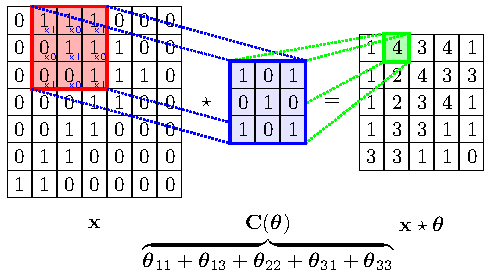
\includegraphics[width=0.7\linewidth]{figures/2d_conv.pdf}
     \caption{图像 $\vec{x}$ 与滤波器 $\vec{C}(\boldsymbol{\theta})$ 进行卷积的过程。滤波器参数 $\boldsymbol{\theta}$ 可以表示为生成元 $\boldsymbol{\theta}_{vw}$ 的线性组合。}
     \label{fig:2dconv}
\end{figure}
\begin{equation}\mathbf{F}(\mathbf{x})_{uv}= \sum_{a=1}^{H^f}\sum_{b=1}^{W^f} {\alpha}_{ab} x_{u+a, v+b}~.
\end{equation}
也可以选择其他基 $\boldsymbol{\theta}_{vw}$，它们将产生等价的运算（但 $\alpha_{vw}$ 的选择可能不同）。一个常见例子是把\emph{方向导数} $\thetab_{vw}(u_1,u_2) = \delta(u_1, u_2) - \delta(u_1-v,u_2-w), (v,w) \neq (0,0) $ 与局部平均 $\thetab_{0}(u_1,u_2) = \frac{1}{H_fW_f}$ 一并使用。事实上，方向导数可以看作图上扩散过程在网格上的对应物：若假设每个像素都是与网格中相邻像素相连的节点，便可恢复这一对应关系。

当标量输入通道替换为多个通道（例如 RGB 颜色通道，或更一般地，任意数量的\emph{特征图}）时，卷积滤波器就成为一个{\em 卷积张量}，表示输入特征到输出特征图的任意线性组合。在坐标表示下，可以写为
%
\begin{equation}
\label{eq:basiccnnlayer}
\mathbf{F}(\mathbf{x})_{uvj}= \sum_{a=1}^{H^f}\sum_{b=1}^{W^f}\sum_{c=1}^M {\alpha}_{jabc} x_{u+a, v+b, c}~,~ j\in[N]~,
\end{equation}
%
其中，$M$ 和 $N$ 分别为输入通道数和输出通道数。
这一基本运算涵盖了一大类神经网络架构；下一节将说明，这些架构对计算机视觉、信号处理及其他许多领域产生了深远影响。这里，我们不去逐一剖析 CNN 数量繁多的可能架构变体，而是着重讨论促使其得到广泛应用的一些关键创新。



\paragraph{高效的多尺度计算}
正如一般对称性的 GDL 模板所讨论的，从卷积算子 $\mathbf{F}$ 中提取平移不变特征需要一个非线性步骤。\marginnote{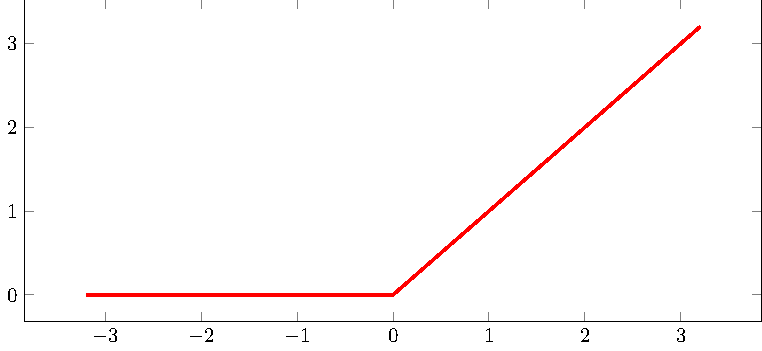
\includegraphics[width=\linewidth]{figures/relu.pdf}\\ ReLU 常被视为一种“现代”架构选择，但早在 Neocognitron 中就已使用 \citep{fukushima1982neocognitron}。整流等价于解调原理；解调是电气工程的基础，支撑了 FM 广播等多种传输协议，在神经元活动模型中也具有重要作用。}%so that the energy captured along each sub-band $\thetab_{ij}$ is mapped towards the low-frequencies
卷积特征通过一个非线性的%rectification stage,
\emph{激活函数} $\sigma$ 处理；该函数逐元素作用于输入，即 $\sigma: \gX(\Omega) \to \gX(\Omega)$，且 $\sigma(\mathbf{x})(u) = \sigma(\mathbf{x}(u))$。写作本文时最流行的例子或许是修正线性单元（ReLU）：$\sigma(x) = \max(x, 0)$。%, or other choices of activation function.
这种非线性会有效地对信号进行\emph{整流}，将其能量推向较低频率，并通过迭代这一构造，使跨尺度的高阶交互计算成为可能。

早在 \cite{fukushima1982neocognitron} 和 \cite{lecun1998gradient} 的早期工作中，CNN 及类似架构
%Since the early days from Fukushima and LeCun, CNN architectures 
就已经采用多尺度结构：在每个卷积层（\ref{eq:basiccnnlayer}）之后执行一次网格粗化
$\mathbf{P} : \gX(\Omega) \to \gX(\Omega')$，其中网格 $\Omega'$ 的分辨率比 $\Omega$ 更粗。
这使多尺度滤波器能够有效增大感受野，同时保持每个尺度上的参数数量恒定。
%
可以采用多种信号粗化%or
策略 $\mathbf{P}$（称为\emph{池化}），其中最常见的是%possible: either %by %explicitly
先应用低通抗混叠滤波器（如局部平均），再对网格下采样，或者采用非线性最大池化。
%
%
%Inspired by neuroscience, 

总之，一个“基础”CNN 层可以表示为几何深度学习蓝图中已经引入的基本对象之复合：
\begin{equation}
    \mathbf{h} = \mathbf{P}(\sigma(\mathbf{F}( \mathbf{x})))~,
\end{equation}
即等变线性层 $\mathbf{F}$、粗化运算 $\mathbf{P}$ 和非线性函数 $\sigma$。还可以在 CNN 中执行平移不变的\emph{全局}池化运算。直观地说，每个像素在若干次卷积后都概括了一个以自身为中心的\emph{斑块}，并据此\emph{提出}图像的最终表示\marginnote{仅由本段所述运算组成的 CNN 常称为“全卷积”网络。相比之下，许多 CNN 在应用足够多的等变层和粗化层后，会沿空间轴\emph{展平}图像并将其传给 MLP 分类器；这样会失去平移不变性。}；最终选择由某种对这些提议的聚合方式决定。平均函数是一种常见选择，因为无论图像大小如何，其输出都能保持相近的量级 \citep{springenberg2014striving}。

图 \ref{fig:cnn_drawn_plot} 展示了遵循这一 CNN 蓝图的若干著名实例，其中一些将在下文讨论。

\begin{figure}
    \centering
    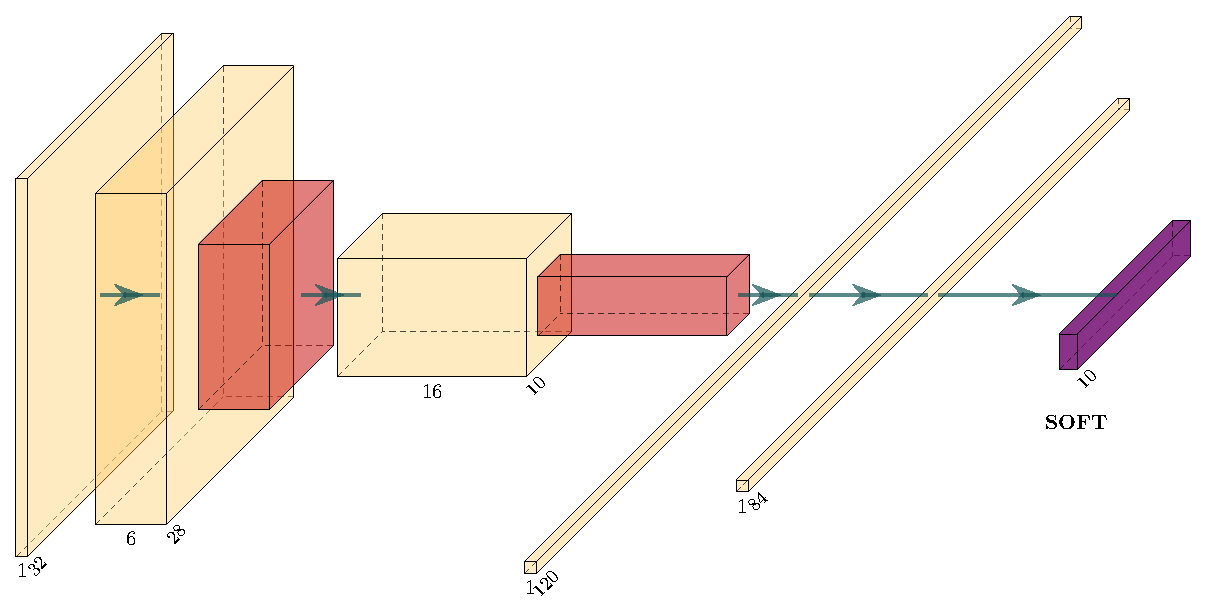
\includegraphics[width=0.85\textwidth]{figures/lenet.pdf}
    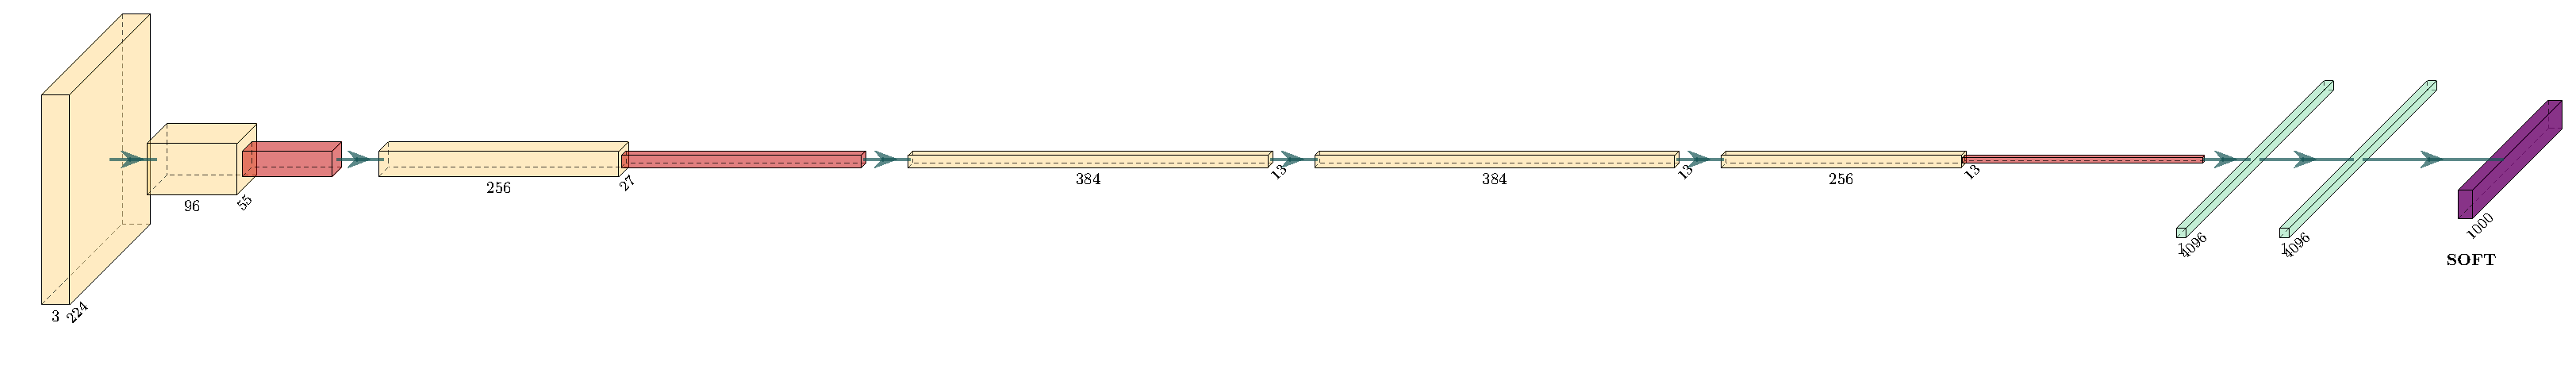
\includegraphics[width=0.85\textwidth]{figures/alexnet.pdf}
    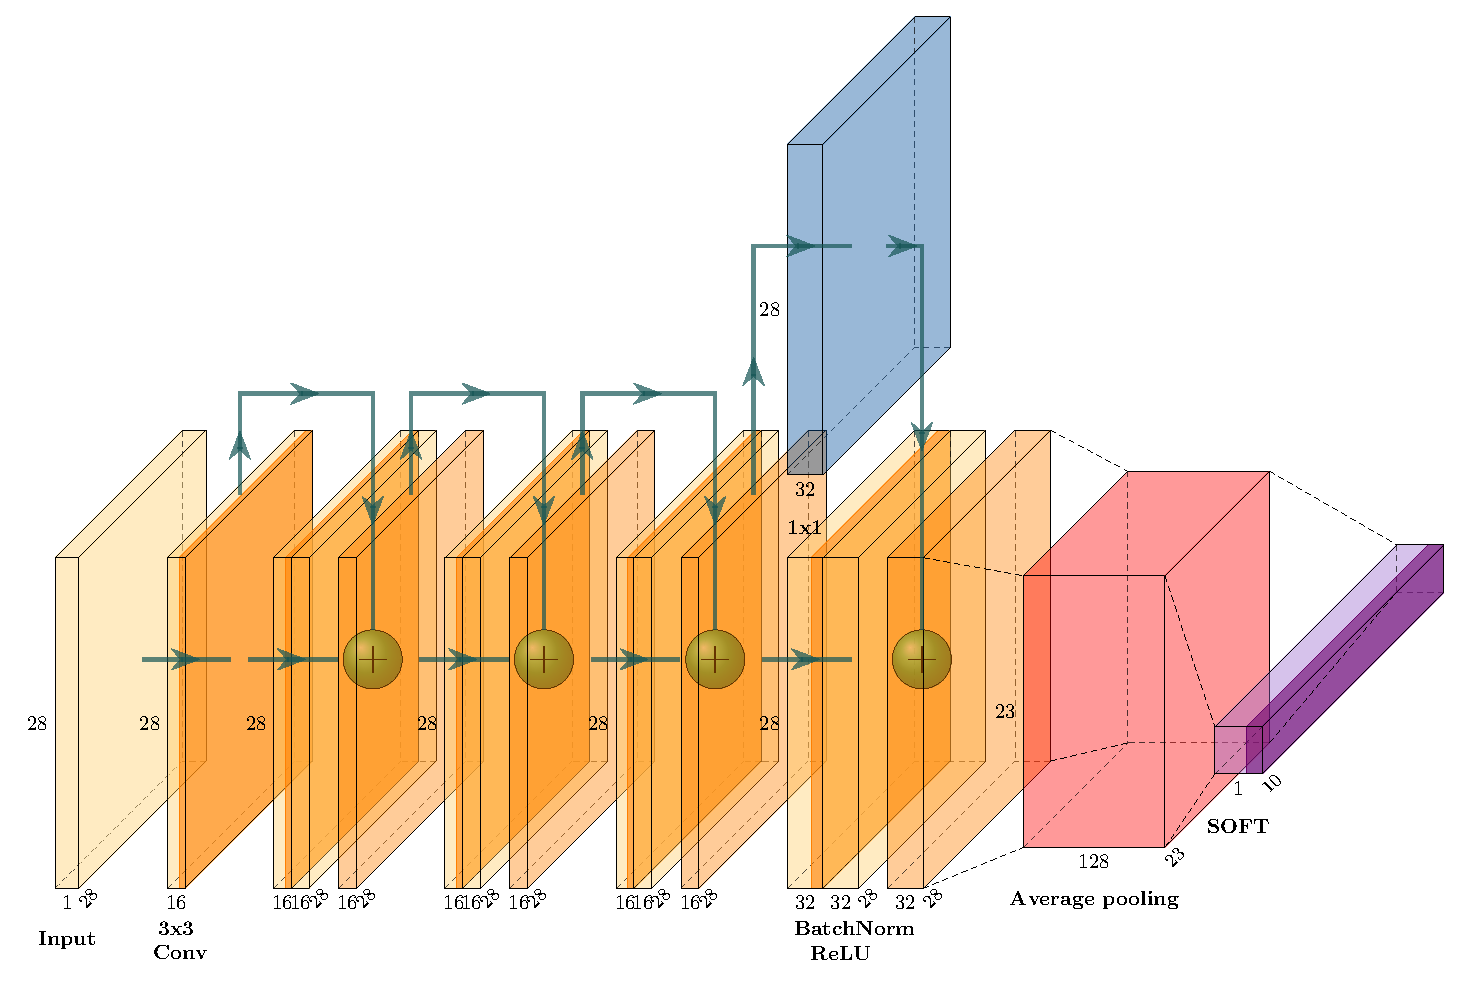
\includegraphics[width=0.85\textwidth]{figures/resnet.pdf}
    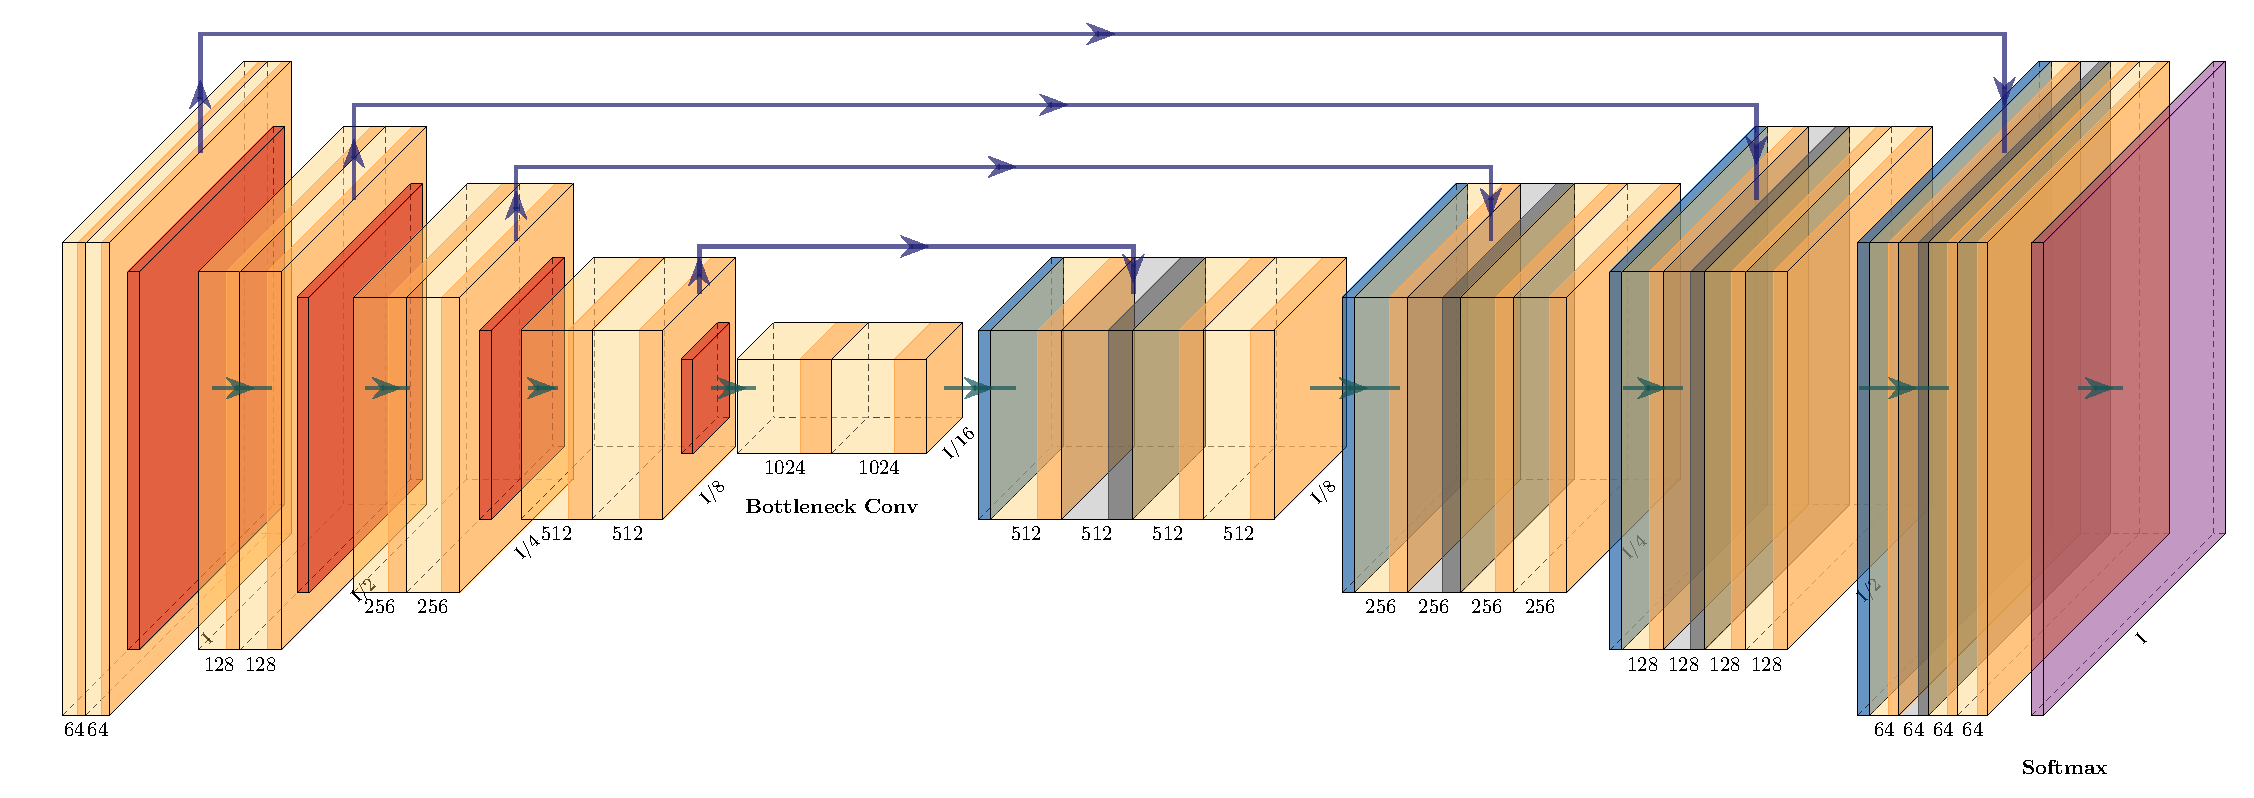
\includegraphics[width=0.85\textwidth]{figures/Unet.pdf}
    \caption{著名的 CNN 架构实例。\textbf{从上到下}：LeNet \citep{lecun1998gradient}、AlexNet \citep{krizhevsky2012imagenet}、ResNet \citep{he2016deep} 和 U-Net \citep{ronneberger2015u}。使用 PlotNeuralNet 包绘制 \citep{haris2018}。}
    \label{fig:cnn_drawn_plot}
\end{figure}
%role of depth
\paragraph{深层网络与残差网络}
因此，在最简单的形式下，CNN 架构由超参数\linebreak[4] $(H^f_k, W^f_k, N_k, p_k )_{k \leq K}$ 指定，其中 $M_{k+1} = N_k$，而 $p_k=0,1$ 表示是否执行网格粗化。虽然这些超参数在实践中都很重要，但一个尤其重要的问题是理解深度 $K$ 在 CNN 架构中的作用，以及选择这一关键超参数所涉及的基本权衡，特别是它与滤波器大小（$H_k^f, W_k^f$）之间的关系。

尽管这一问题尚无严格答案，近年来不断积累的经验证据表明，更深（$K$ 较大）而更窄（$(H^f_k, W^f_k)$ 较小）的模型具有更有利的权衡\marginnote{
从历史上看，ResNet 模型之前已有\emph{高速公路网络} \citep{srivastava2015highway}，后者允许用更一般的\emph{门控}机制控制残差信息流。}。在这一背景下，\cite{he2016deep} 的关键洞见是对每个卷积层重新参数化，使其建模前一层特征的\emph{扰动}，而不是一般的非线性变换：
\begin{equation}
    \mathbf{h} = \mathbf{P}\left(\mathbf{x} + \sigma(\mathbf{F}(\mathbf{x})) \right)~.
\end{equation}
由此得到的\emph{残差}网络相较前一种表述具有若干关键优势。本质上，残差参数化与如下观点一致：深度网络是底层连续动力系统的离散化，而该系统由常微分方程（ODE）建模\marginnote{在这种情况下，ResNet 正在对 ODE 执行前向 Euler 离散化：$\dot{\mathbf{x}} = \sigma( \mathbf{F}(\mathbf{x}))$。}。关键在于，事实证明，通过建模速度来学习动力系统远比直接学习其位置容易。在我们的学习设定中，这意味着优化景观具有更有利的几何形态，因而能够训练比以往深得多的架构。正如未来工作将讨论的那样，使用深度神经网络进行学习定义了一个非凸优化问题；在某些简化情形下，该问题可以用梯度下降方法高效求解。ResNet 参数化的关键优势已经在简单情形中得到严格分析 \citep{hardt2016identity}，并且仍是理论研究的活跃方向。
最后，Neural ODE \citep{chen2018neural} 是近期一种流行架构，它直接学习 ODE $\dot{\mathbf{x}} = \sigma( \mathbf{F}(\mathbf{x}))$ 的参数并依赖标准数值积分，从而进一步推进了与 ODE 的类比。

%\michael{This is also the case for GNNs, which are a discretization of a nonlinear diffusion PDE} \petar{skipping for now, as discussed with Michael}

%Normalization 
\paragraph{归一化}
另一个显著提升 CNN 经验性能的重要算法创新是\emph{归一化}。早期的神经活动模型假设，神经元会执行某种形式的局部“增益控制”，其中层系数 $\mathbf{x}_{k}$ 被替换为 $\mathbf{\tilde{x}}_{k} = \sigma_k^{-1} \odot (\mathbf{x}_{k} - \mu_k)$。这里，$\mu_k$ 和 $\sigma_k$ 分别编码 $\mathbf{x}_k$ 的一阶矩与二阶矩信息；它们既可以全局计算，也可以局部计算。

在深度学习中，这一原理通过\emph{批归一化}层 \citep{ioffe2015batch} 得到广泛采用\marginnote{需要指出的是，在批归一化出现以前，对神经网络激活进行归一化就已经受到关注；例如见 \cite{lyu2008nonlinear}。}，随后又产生了若干变体 \citep{ba2016layer,salimans2016weight,ulyanov2016instance,cooijmans2016recurrent,wu2018group}。
尽管已有工作试图从条件更良好的优化景观角度严格解释归一化的益处 \citep{santurkar2018does}，但在写作本文时，仍然缺少能够提供指导原则的一般理论。

\paragraph{数据增强}
CNN 虽然编码了与平移不变性和尺度分离相关的几何先验，却没有显式考虑其他已知的语义保持变换，例如光照或颜色变化，以及小幅旋转和缩放。以最小架构改动纳入这些先验的一种实用方法是进行\emph{数据增强}，即手动对输入图像施加上述变换，并把所得图像加入训练集。

数据增强在经验上取得了成功并得到广泛应用：它不仅用于训练最先进的视觉架构，还推动了自监督表示学习和因果表示学习的多项发展 \citep{chen2020simple,grill2020bootstrap,mitrovic2020representation}。然而，从样本复杂度看，它已被证明是次优的 \citep{mei2021learning}；更高效的策略是考虑具有更丰富不变群的架构，这正是下文要讨论的内容。

%TODO: discuss Preserving Orientation: contrast this with the GNN setting. 

% ====

% To define a convolutional operator, we will consider the case of 2D inputs (i.e. single-channel images), $\vec{X}\in\mathbb{R}^{h\times w}$. Let $\vec{K}\in\mathbb{R}^{n\times m}$ be a small \emph{kernel matrix} (typically, $n = m = 3$ in modern neural network architectures). The kernel is overlaid in all possible ways
% over the input (see Figure \ref{fig:2dconv}), recording sums of elementwise products to create a
% new image, $\vec{X}'$:\marginnote{It should be noted that this approach is actually cross‐correlation rather than the convolution; but, for purposes of machine learning, the two are equivalent.}
% \begin{equation}
%     x'_{ab} = \sum_{i=1}^n\sum_{j=1}^m k_{ij}x_{a+i-1,b+j-1}
% \end{equation}
% The image is typically padded with sufficiently many zeroes on the edges, to ensure that the size of the output matches the size of the input.

% Moving from here to a convolutional \emph{layer} requires a few extensions. If the input has multiple channels, the kernel matrix is \emph{extended} in the channel dimension to match the input. This \emph{kernel tensor} specifies a single output channel. Each output channel requires a separate kernel tensor. Lastly, a channel‐specific bias and nonlinearity may be applied to obtain the final output image (sometimes known as a \emph{feature map}). 

% In summary, to process an input image $\vec{X} \in \mathbb{R}^{h\times w\times d}$ using a convolutional layer computing $d'$ channels, we require a kernel tensor $\vec{K}\in\mathbb{R}^{n\times m\times d\times d'}$ and a bias vector $\vec{b}\in\mathbb{R}^{d'}$, and proceed as follows:\marginnote{\includegraphics[width=\linewidth]{figures/fullconv.png}}
% \begin{equation}
%     x'_{abc} = \sigma\left(b_c + \sum_{i=1}^n\sum_{j=1}^m\sum_{k=1}^d k_{ijkc}x_{a+i-1,b+j-1,k}\right)
% \end{equation}

% This layer clearly exploits the structure present in an image, with neighbouring pixels
% influencing each other far more strongly than ones on opposite corners. The operator is
% also \emph{translation equivariant}, as required for grids: as the same kernels are applied identically across each image patch, we are encoding a structural bias that a feature of interest is important, no matter where it occurs in the image.

% Often, we are interested in computing outputs on the level of \emph{entire} images. Hence it is useful to compress an image to a \emph{flat} representation, but doing so on the input image sizes often results in an overly large vector (of size $O(hwd)$. Accordingly, once a sufficient number of convolutions has been applied to the input, it is very common to \emph{downsample} the image. 

% As convolutions \emph{``light up''}\marginnote{\includegraphics[width=\linewidth]{figures/maxpool.png}} (return high values) when a certain
% pattern of interest is detected in the input, when summarising the image it makes sense
% to preserve \emph{maximally activated} components of it. This motivates the \emph{max‐pooling} layer, which takes $n\times m$ (usually disjoint, with $n = m = 2$) image patches across each channel and summarises them by taking only the maximal pixel value.

% \michael{This is certainly not the most important reason for using nonlinear pooling - I think we want to refer to Bruna, Mallat 2012 here}

% \begin{figure}
%     \centering
%     \includegraphics[width=\linewidth]{figures/fig_conv.png}
%     \caption{An overview of a typical CNN architecture for image classification. Convolutional and pooling layers are interleaved, with the depth (number of features computed per pixel) increased at the expense of height and width. Once the images are small enough, they are flattened into 1D, and an MLP is used to classify them.}
%     \label{fig:figconv}
% \end{figure}

% Note that a $2\times 2$ max‐pooling layer (which is most common) will preserve only a quarter of the pixels, while leaving the channel axis unchanged. This provides more space
% for gradually increasing the channel size, and therefore computing a richer quantity of
% higher‐level features. A typical convolutional neural network architecture thus consists
% of a series of interleaved convolutional and pooling layers, until the input is reduced sufficiently to be processed by an MLP---as in Figure \ref{fig:figconv}.

% It is also possible, though less common, to perform \emph{global} pooling operations within CNNs. Intuitively, this involves each pixel---which, after several convolutions, summarises a \emph{patch} centered around it---\emph{proposing} the final representation of the image, with the ultimate choice being guided by a form of aggregation of these proposals. A popular choice here is the average function, as its outputs will retain similar magnitudes irrespective of the image size \citep{springenberg2014striving}.

% It is generally perceived that, for image recognition tasks, deep convolutional networks
% strongly draw their outperformance from both their depth \textbf{and} their parameter tying. However, training very deep convolutional networks used to be notoriously difficult. As shown by \citet{he2016deep}, overly deep convolutional networks \emph{do not overfit}, as their training performance degrades along with their testing performance. This is somewhat counterintuitive, as increased depth not only comes with larger parameter spaces to optimise, but moreover, if the additional layers are useless to learning good representations,
% the layer could simply choose to \emph{ignore} them (by learning the \textbf{identity} function).

% Through this counterintuitive property, the authors proposed an obvious fix: the \emph{residual (skip) connection} \citep{he2016deep}, which ``shortcuts'' a particular block of operations in a neural
% network. If a neural network block computes a function $f(\vec{x})$, a skip connection allows $\vec{X}$ to directly reach the output of this block through aggregation; i.e. the neural network simply computes $f(\vec{x}) + \vec{x}$. More generally, if the block changes the input dimensionality, a simple linear projection may be introduced to correct for this:
% \begin{equation}
%     \widetilde{f}(\vec{x}) = f(\vec{x}) + \vec{W}_\mathrm{skip}\vec{x} 
% \end{equation}
% Note that, effectively, this operation allows signals to directly reach deeper stages of the
% input processing, and therefore allows the network to choose its own depth. This turned
% out to be a very powerful and versatile concept, that enabled a 152‐layer network to win
% the ImageNet competition in 2015. Currently, it is ubiquitous in deep learning. It is worth noting that such (``ResNet'') models are predated by \emph{highway networks} \citep{srivastava2015highway}, which allow for more general \emph{gating} mechanisms to control the residual information flow.

% \michael{Scale separation and pooling - show here how pooling makes approximate translation invariance?}





\subsection{群等变 CNN}

正如第 \ref{sec:groups} 节所讨论的，我们可以把卷积运算从欧氏空间上的信号推广到任意\emph{齐性空间} $\Omega$ 上的信号，其中群 $\fG$ 作用于该空间\marginnote{回顾一下，齐性空间是配备传递群作用的集合 $\Omega$；这意味着对于任意 $u,v \in \Omega$，都存在 $\fg \in \fG$ 使得 $\fg. u = v$。}。
在欧氏卷积中，经过{\em 平移的}滤波器会与信号进行匹配；与此类似，群卷积的思想是利用群作用在域上移动滤波器，例如对其进行旋转和平移。
借助群作用的\emph{传递性}，我们可以把滤波器移动到 $\Omega$ 上任意位置。
本节将讨论群卷积这一一般思想的若干具体实例，包括实现细节和架构选择。

%, including discrete roto-translation equivariant planar and 3D CNNs, convolutions on the group of symmetries of a DNA sequence, and spherical CNNs.

\paragraph{离散群卷积}

我们先考虑域 $\Omega$ 和群 $\fG$ 都是离散的情形。
%
第一个例子是表示为三维网格上信号的医学体数据图像%(e.g. medical scans)
，它具有离散平移和旋转对称性。%,
%and DNA sequences with translation symmetry as well as so-called \emph{reverse-complement} symmetry (explained below).
%
%For the first example, we take as 
域是三维立方网格 $\Omega = \Z^3$，而图像（例如
MRI 或 CT 三维扫描）被建模为函数 $x : \Z^3 \rightarrow \R$，即 $x \in \mathcal{X}(\Omega)$。
尽管实践中这类图像的支撑位于有限长方体 $[W] \times [H] \times [D] \subset \Z^3$ 上，我们仍倾向于把它们看作 $\Z^3$ 上经过适当零填充的函数。
%that happen to be zero outside a finite region. 
%
作为对称性，我们考虑群 $\fG = \Z^3 \rtimes O_h$，它由 $\Z^3$ 上保持距离和定向的变换组成。
该群由平移（$\Z^3$）和离散旋转 $O_h$ 组成，后者由绕三个坐标轴的 $90$ 度旋转生成（见图 \ref{fig:cayley-diagram-Oh}）。

\begin{figure}[h!]
    \centering
    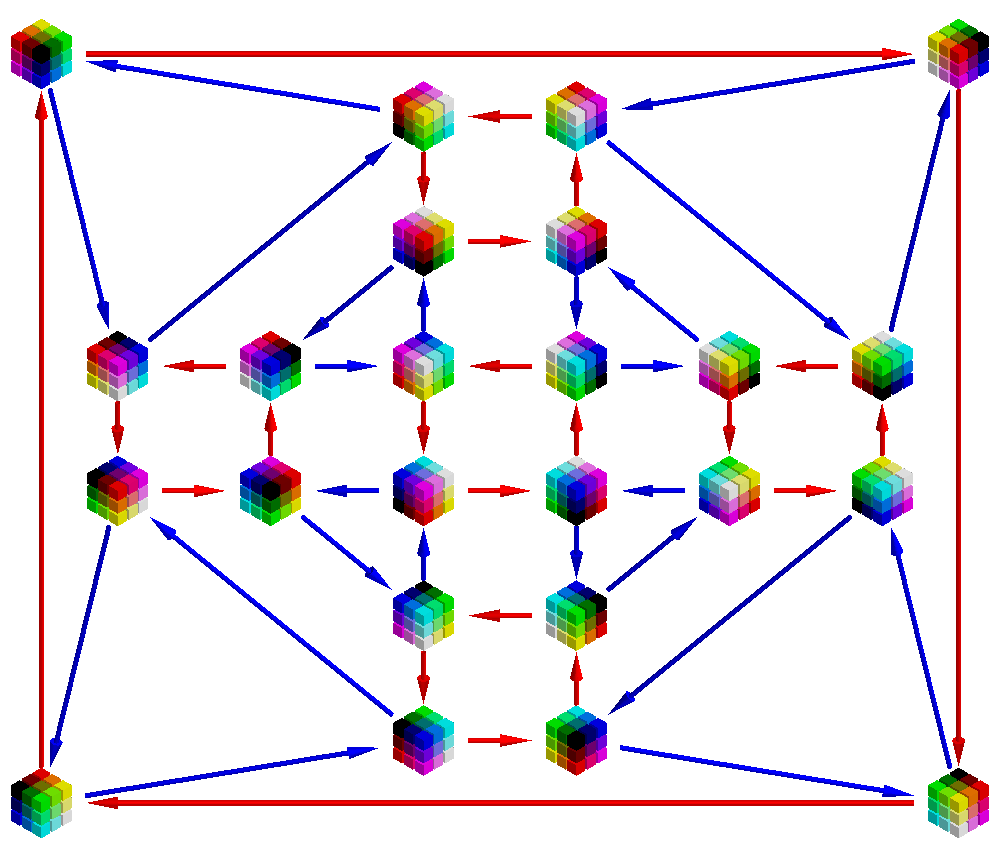
\includegraphics[width=0.6\textwidth]{figures/Oh}
    \caption{一个 $3 \times 3$ 滤波器经全部 $24$ 个离散旋转群元素 $O_h$ 旋转后的结果；该群由绕竖直轴的 $90$ 度旋转（红色箭头）和绕对角轴的 $120$ 度旋转（蓝色箭头）生成。
    %The diagram shown here (where each node is associated with a group element, and each arrow with a generator), is known as the {\em Cayley diagram}.
    }
    \label{fig:cayley-diagram-Oh}
\end{figure}

第二个例子考虑 DNA\marginnote{DNA 是一种生物聚合物分子，
%carrying the generic instructions responsible for the development and functioning of all currently known life forms. It is 
由称为{\em 核苷酸}的四种重复单元（胞嘧啶、鸟嘌呤、腺嘌呤和胸腺嘧啶）组成。它们排列成两条相互缠绕的双螺旋链，每种核苷酸都与其互补核苷酸相对（{\em 碱基对} A/T 和 C/G）。} 序列，它由 C、G、A 和 T 四个字母组成。
%
这些序列可以在一维网格 $\Omega = \Z$ 上表示为信号 $x : \Z \rightarrow \R^4$，其中每个字母在 $\R^4$ 中采用 one-hot 编码。
自然地，该网格具有离散的一维平移对称性，但 DNA 序列还具有一种有趣的额外对称性。
这种对称性源于 DNA 以双螺旋形式存在的物理方式，以及细胞分子机器读取它的方式。
%
%Recall that a DNA molecule forms a double helix, with each nucleotide base occurring opposite one of the complementary type: A and T are complementary, as are C and G.
双螺旋的每条链都从所谓的 $5'$ 端开始，以 $3'$ 端结束；一条链上的 $5'$ 端与另一条链上的 $3'$ 端互补。
换言之，两条链的定向相反。\marginnote{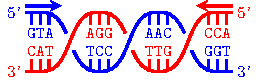
\includegraphics[width=\linewidth]{figures/tikz_dna.pdf}\\ DNA 双螺旋结构示意图，两条链分别以蓝色和红色表示。注意，螺旋中的序列彼此互补，且读取方向相反（从 5' 到 3'）。}
%{ (see Figure TODO (optional))}.
由于 DNA 分子总是从 $5'$ 端开始读取，而我们并不知道从哪一条链读取，因此像 ACCCTGG 这样的序列等价于将其反向并把每个字母替换为互补字母后得到的序列 CCAGGGT。
这称为字母序列的{\em 反向互补对称性}。
因此，我们得到二元素群 $\Z_2 = \{0, 1\}$，其中恒等变换对应于 $0$，反向互补变换对应于 $1$（复合运算满足 $1 + 1 = 0 \mod{2}$）。
完整的群结合了平移与反向互补变换。



在我们的情形中，
第 \ref{sec:groups} 节定义的群卷积~(\ref{eq:group-conv}) 可写为
%is defined as:
\begin{equation}
    (x \star \theta)(\fg) = \sum_{u \in \Omega} x_u \rho(\fg) \theta_u,
\end{equation}
它是（单通道）输入信号 $x$ 与滤波器 $\theta$ 的内积；滤波器由 $\fg \in \fG$ 通过 $\rho(\fg) \theta_u = \theta_{\fg^{-1} u}$ 进行变换，而输出 $x\star \theta$ 是 $\fG$ 上的函数。
注意，由于 $\Omega$ 是离散的，我们把式~(\ref{eq:group-conv}) 中的积分替换成了求和。%\michael{Define: what is the size of $\rho(\fg)$?} \petar{I think it depends on whether we're doing DNA conv or rotation conv.}


\paragraph{变换+卷积方法}
我们将说明，群卷积可以分两步实现：滤波器变换步骤和平移卷积步骤。
滤波器变换步骤为基本滤波器创建旋转（或反向互补变换）副本，而平移卷积与标准 CNN 中相同，因而可以在 GPU 等硬件上高效计算。%highly optimized.
为说明这一点，注意在两个例子中，我们都可以把一般变换 $\fg \in \fG$ 写成先进行变换 $\fh \in \fH$（例如旋转或反向互补变换），再进行平移 $\fk \in \Z^d$，即 $\fg = \fk \fh$（并置表示群元素 $\fk$ 和 $\fh$ 的复合）。
由群表示的性质，% $\rho$ is a representation,
可得 $\rho(\fg) = \rho(\fk \fh) = \rho(\fk) \rho(\fh)$。
因此，%we have
\begin{equation}
    \begin{aligned}
        (x\star \theta )(\fk \fh) 
        &=
        \sum_{u \in \Omega} x_u \rho(\fk) \rho(\fh) \theta_{u} \\
        &=
        \sum_{u \in \Omega} x_u (\rho(\fh) \theta)_{u - \fk}
    \end{aligned}
\end{equation}
%\michael{is the filter reversed here? }
可以看出，最后一个等式正是信号 $x$ 与变换后滤波器 $\rho(\fh) \theta$ 的标准（平面欧氏）卷积。
因此，为了对这些群实现群卷积，我们取规范滤波器 $\theta$，创建变换后的副本 $\theta_\fh = \rho(\fh) \theta$，每个 $\fh \in \fH$ 对应一个副本（例如每个旋转 $\fh \in O_h$ 或 DNA 反向互补对称性 $\fh \in \Z_2$），然后用 $x$ 分别与这些滤波器卷积：$(x\star \theta )(\fk \fh)  = (x\star \theta_{\fh} )(\fk)$。
在两个例子中，对称性都只是通过置换滤波器系数作用于滤波器，离散旋转的情形如图 \ref{fig:cayley-diagram-Oh} 所示。
因此，这些运算可以使用预先计算索引的索引操作高效实现。


尽管我们把群卷积 $x \star \theta$ 输出的特征图定义为 $\fG$ 上的函数，但由于 $\fg$ 可以分解为 $\fh$ 和 $\fk$，也可以把它们看作一组堆叠的欧氏特征图（有时称为\emph{定向通道}），每个滤波器变换/定向 $\fk$ 对应一个特征图。
例如，在第一个例子中，我们会为每个滤波器旋转（图 \ref{fig:cayley-diagram-Oh} 中的每个节点）关联一个特征图，该特征图通过
%translationally 
以传统平移意义对旋转后的滤波器进行卷积而得到。
因此，这些特征图仍可存储为 $W \times H \times C$ 数组，其中通道数 $C$ 等于独立滤波器的数量乘以变换 $\fh \in \fH$（例如旋转）的数量。

如第 \ref{sec:groups} 节所示，群卷积是等变的：$(\rho(\fg) x) \star \theta = \rho(\fg) (x \star \theta)$。
就定向通道而言，这意味着在 $\fh$ 的作用下，每个定向通道都会发生变换，而各定向通道本身也会被置换。
例如，若对图 \ref{fig:cayley-diagram-Oh} 中的每个变换关联一个定向通道，并施加绕 z 轴 $90$ 度的旋转（对应红色箭头），特征图就会按照红色箭头所示进行置换。
%
上述描述清楚表明，群卷积神经网络与传统 CNN 十分相似。
因此，第~\ref{sec:cnnsec} 节讨论的许多网络设计模式（例如残差网络）也可以与群卷积结合使用。




\paragraph{Fourier 域中的球面 CNN}
对于第~\ref{sec:groups} 节所见的球面连续对称群，可以使用适当的 Fourier 变换在谱域中实现卷积（提醒读者，$\mathbb{S}^2$ 上的卷积是 $\mathrm{SO}(3)$ 上的函数，因此要实现多层球面 CNN，需要在这两个域上都定义 Fourier 变换）。
%
%The analogy of the Fourier basis on 
{\em 球谐函数}是二维球面上的一组正交基，类似于由复指数函数构成的经典 Fourier 基。
%
在特殊正交群上，Fourier 基称为 {\em Wigner D-functions}。%
在这两种情形中，Fourier 变换（系数）都通过与基函数取内积来计算，并且卷积定理的对应形式成立：可以把 Fourier 变换逐元素相乘，从而在 Fourier 域中计算卷积。
%
此外，还存在类 FFT 算法，可高效计算 $\mathbb{S}^2$ 和 $\mathrm{SO}(3)$ 上的 Fourier 变换。更多细节见 \cite{cohen2018spherical}。



%On the $\mathrm{SO}(3)$ group, the Fourier decomposition takes the form 
%$$
%f(\mathbf{R}) = \sum_{l\geq 0} (2l+1) \sum_{i=-l}^{+l} \sum_{j=-l}^{+l} \hat{f}_{l,ij} D_{l,ij}(\mathbf{R})
%$$
%where the Fourier coefficients are defined as %inner products 
%$$
%\hat{f}_{l,ij} = \int_{\mathrm{SO}(3)} f(\mathbf{R}) \overline{D_{l,ij}(\mathbf{R})}\mathrm{d}\mathbf{R}. 
%$$
%The basis functions $D_{l,ij}(\mathbf{R})$ are called the {\em Wigner D-functions}, indexed by the degree $l\geq 0$ and order $i,j = -l, \hdots, +l$, and can be considered as complex matrix-valued functions $\mathbf{D}_l : \mathrm{SO}(2) \rightarrow \mathbb{C}^{(2l+1)\times (2l+1)}$. 
%% \paragraph{Steerability}
%





\subsection{图神经网络}\label{sec:gnn-intro}

%[MOVED from 1.3]

%since graphs exhibit less restrictive geometries and invariances, they invite for the most flexible class of architectures---the \emph{Graph Neural Networks} (GNN). As we will see, all of the neural architectures we will study in this book can be understood as a special case of the GNN, with injected additional geometric constraints and invariances.

%The general concept of constructing {\em permutation equivariant} functions operating over graphs as shared {\em permutation invariant} functions operating over local neighbourhoods appears to be very powerful and underlies the design of most Graph Neural Networks. Under various guises, this local function $g$ can be referred to as ``diffusion'', ``propagation'', or ``message passing''. 
%
%If we are interested in a graph-level output, a common recipe is to construct the latent node features using a {\em permutation equivariant} function $f$, followed by a {\em permutation invariant} function $h$ over the entries of $f({\bf X}, {\bf A})$ to obtain an ordering-independent output. In this context, the function $h$ is often referred to as ``readout'' or ``global pooling''.




%====

图神经网络（GNN）利用置换群的性质，在图上实现了我们的几何深度学习蓝图。GNN 是目前最一般的深度学习架构类别之一；正如本文将说明的，大多数其他深度学习架构都可以理解为带有额外几何结构的 GNN 特例。


按照第 \ref{sec:proto-graphs} 节的讨论，我们认为一个图由邻接矩阵 $\mathbf{A}$ 和节点特征 $\mathbf{X}$ 指定。
%
%
我们将研究如下 GNN 架构：它们是{\em 置换等变}函数 $\mathbf{F}(\mathbf{X},\mathbf{A})$，通过在局部邻域上应用共享的{\em 置换不变}函数 $\phi(\mathbf{x}_u, \mathbf{X}_{\mathcal{N}_u})$ 构造而成。在不同表述中，这一局部函数 $\phi$ 可称为“扩散”“传播”或“消息传递”，而这种 $\mathbf{F}$ 的整体计算则称为“GNN 层”。


在写作本文时，GNN 层的设计与研究是深度学习最活跃的领域之一，因而其研究版图难以梳理。所幸，我们发现绝大多数文献都可以从 GNN 层的三种“类型”（图 \ref{fig:gc_flavours}）推导出来，下面将予以介绍。这些类型决定了 $\phi$ 对邻域特征进行变换的程度，从而允许以不同复杂度建模图上的交互。


在这三种类型中，来自 $\vec{X}_{\mathcal{N}_u}$ 的特征（可能借助某个函数 $\psi$ 进行变换）会由置换不变函数 $\bigoplus$ 进行\emph{聚合}；随后，节点 $u$ 的特征由某个函数 $\phi$ {\em 更新}，从而保证置换不变性。通常，\marginnote{最常见的情形是，$\psi$ 和 $\phi$ 是带激活函数的可学习仿射变换；例如 $\psi(\vec{x}) = {\bf W}\vec{x} + \vec{b}$；$\phi(\vec{x}, \vec{z}) = \sigma\left({\bf W}\vec{x} + {\bf U}\vec{z} + \vec{b}\right)$，其中 ${\bf W}, {\bf U}, \vec{b}$ 是可学习参数，而 $\sigma$ 是修正线性单元等激活函数。$\vec{x}_u$ 作为 $\phi$ 的额外输入，表示一个可选的{\em 跳跃连接}，这通常非常有用。}$\psi$ 和 $\phi$ 是可学习的，
%$\fdef{\bigoplus}{\mathcal{P}(\mathbb{R}^k)}{\mathbb{R}^{k'}}$. 
%
而 $\bigoplus$ 则实现为求和、均值或最大值等非参数运算，不过也可以使用循环神经网络等方式构造 \citep{murphy2018janossy}。


\begin{figure}
    \centering
    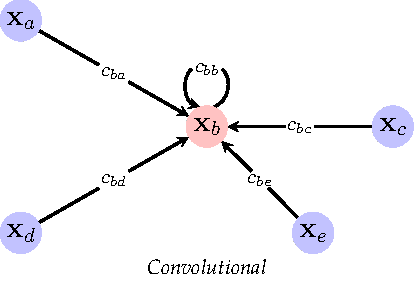
\includegraphics[width=0.33\linewidth]{figures/GNN_GDL_TYPES_C.pdf}
    \hspace{-0.5em}
    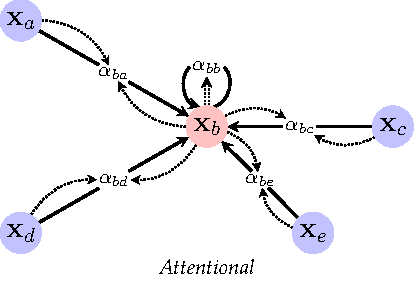
\includegraphics[width=0.33\linewidth]{figures/GNN_GDL_TYPES_A.pdf}
    \hspace{-0.5em}
    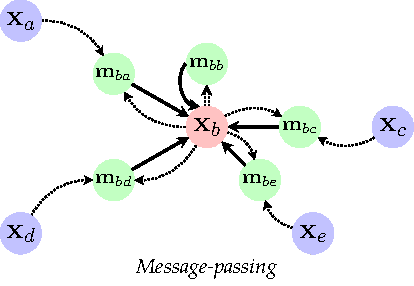
\includegraphics[width=0.33\linewidth]{figures/GNN_GDL_TYPES_MP.pdf}
    \caption{三种 GNN 层类型 $g$ 的数据流可视化。我们用图 \ref{fig:gc_gdl} 中节点 $b$ 的邻域加以说明。从左到右分别为：\textbf{卷积型}，其中发送节点特征乘以常数 $c_{uv}$；\textbf{注意力型}，其中该乘子通过接收节点对发送节点的注意力机制\emph{隐式}计算：$\alpha_{uv}=a(\vec{x}_u, \vec{x}_v)$；以及\textbf{消息传递型}，其中基于发送节点和接收节点共同计算向量消息：$\vec{m}_{uv}=\psi(\vec{x}_u, \vec{x}_v)$。}
    \label{fig:gc_flavours}
\end{figure}%

%All of the above considered, the three flavours are as follows (Figure \ref{fig:gc_flavours}):



%\begin{itemize}
%\item 
在\textbf{卷积型} \citep{kipf2016semi,defferrard2016convolutional,wu2019simplifying} 中，邻域节点的特征使用固定权重直接聚合：
\begin{equation}
    \vec{h}_u = \phi\left(\vec{x}_u, \bigoplus\limits_{v\in\mathcal{N}_u}c_{uv}\psi(\vec{x}_v)\right).
\end{equation}
这里，$c_{uv}$ 指定节点 $v$ 对节点 $u$ 表示的\emph{重要性}。它是一个常数，通常直接依赖于表示图结构的 ${\bf A}$ 中的元素。
%
注意，当聚合算子 $\bigoplus$ 取为求和时，可以将其视为线性扩散或位置相关的线性滤波，即卷积的推广。\marginnote{值得注意的是，这一类型并不能表示\emph{所有}卷积型（即与图结构可交换的）GNN 层，但涵盖了实践中提出的大多数此类方法。未来工作将给出详细讨论和扩展。}
%
具体而言，第~\ref{sec:manifolds} 节和第~\ref{sec:meshes} 节所见的谱滤波器属于这一类别，因为它们相当于对逐节点信号应用固定局部算子（例如 Laplacian 矩阵）。
 
 
%\michael{Now we discussed spectral filters, so we can add a remark here}

%\item 
在\textbf{注意力型} \citep{velickovic2018graph,monti2017geometric,zhang2018gaan} 中，交互是隐式的：
\begin{equation}
    \vec{h}_u = \phi\left(\vec{x}_u, \bigoplus\limits_{v\in\mathcal{N}_u}a(\vec{x}_u, \vec{x}_v)\psi(\vec{x}_v)\right).
\end{equation}
这里，$a$ 是可学习的\emph{自注意力机制}，用于隐式计算重要性系数 $\alpha_{uv} = a(\vec{x}_u, \vec{x}_v)$。这些系数通常在所有邻居上进行 softmax 归一化。
%
当 $\bigoplus$ 为求和时，聚合结果仍是邻域节点特征的线性组合，但此时权重依赖于特征。


%\item 
最后，\textbf{消息传递型} \citep{gilmer2017neural,battaglia2018relational} 相当于沿边计算任意向量（“消息”）：
\begin{equation}
    \vec{h}_u = \phi\left(\vec{x}_u, \bigoplus\limits_{v\in\mathcal{N}_u}\psi(\vec{x}_u, \vec{x}_v)\right).
\end{equation}
这里，$\psi$ 是可学习的\emph{消息函数}，用于计算节点 $v$ 发送给节点 $u$ 的向量；聚合则可以视为图上的一种消息传递形式。
%\end{itemize}


需要注意的是，这些方法在表示能力上存在包含关系：\emph{卷积} $\subseteq$ \emph{注意力} $\subseteq$ \emph{消息传递}。事实上，注意力型 GNN 可以用实现为查找表 $a(\vec{x}_u, \vec{x}_v) = c_{uv}$ 的注意力机制来表示卷积型 GNN；而卷积型和注意力型 GNN 都是消息传递的特例，其中消息仅包含发送节点的特征：对于卷积型 GNN，$\psi(\vec{x}_u, \vec{x}_v) = c_{uv}\psi(\vec{x}_v)$；对于注意力型 GNN，$\psi(\vec{x}_u, \vec{x}_v) = a(\vec{x}_u, \vec{x}_v)\psi(\vec{x}_v)$。
%

这并不意味着消息传递型 GNN 始终是最有用的变体；由于它们必须沿边计算向量值消息，通常更难训练，并且需要庞大的内存。此外，在许多自然产生的图上，图的边编码了下游类别的相似性（即一条边 $(u, v)$ 意味着 $u$ 和 $v$ 很可能具有相同输出）。对于这种图（常称为\emph{同配图}），无论从正则化还是可扩展性看，在邻域上进行卷积聚合通常都是远为合适的选择。注意力型 GNN 提供了一个“中间方案”：它们能够对邻域内的复杂交互进行建模，同时沿边仅计算标量值，因此比消息传递型更具可扩展性。


这里提出“三种类型”的分类是为了保持简洁，因而不可避免地忽略了 GNN 模型中大量细微差别、洞见、推广和历史背景。尤其是，它不包括基于 Weisfeiler-Lehman 层次结构的高维 GNN，以及依赖显式计算图 Fourier 变换的谱%\marginnote{Though many works make a distinction between ``spatial'' and ``spectral'' GNNs, we find that this distinction is rather artificial and must be taken with a grain of salt. Many proposed spectral filters are expressible in terms of simple matrix operations (e.g. polynomials of the graph Laplacian) and hence boil down to simple spatial operations that fall under the ``convolutional'' flavor presented here.}
GNN。
%
%Such a wealth somewhat uniquely appears in graph representation learning, given the flexible invariances present in graphs, and their ubiquity as a representational tool across the natural and social sciences. 
%We will dedicate Chapter \ref{ch:graphs} to a more careful and detailed exploration of deep learning models for graphs.

%\marginnote{Examples to be covered include: higher-order GNNs, $k$-invariant graph networks, and ``true spectral'' GNNs which rely on the Graph Fourier Transform.}




%We now provide a ``bird's eye'' view of \emph{graph neural networks} (GNNs)---the most popular approach for constructing permutation equivariant neural models over graphs.

%As per Section \ref{sec:proto-graphs}, we will consider a graph  representation learning setup with graphs specified by a matrix of node features, ${\bf X}\in\mathbb{R}^{|V|\times k}$ and an adjacency matrix, ${\bf A}\in\mathbb{R}^{|V|\times |V|}$. Our aim is to construct permutation equivariant functions over these graphs, $\fdef{f}{\mathbb{R}^{|V|\times k} \times \mathbb{R}^{|V|\times |V|}}{\mathbb{R}^{|V|\times k'}}$, such that $f({\bf X}, {\bf A}) = {\bf H}$, where $\vec{x}_i$ and $\vec{h}_i$ are the input and latent features of node $i$. 

%Furthermore, we will construct $f$ through shared application of a local function, $\fdef{g}{\mathbb{R}^k\times \mathcal{P}(\mathbb{R}^k)}{\mathbb{R}^{k'}}$, such that $g(\vec{x}_i, \vec{X}_{\mathcal{N}_i}) = \vec{h}_i$, where $\vec{X}_{\mathcal{N}_i}\in\mathcal{P}(\mathbb{R}^k)$ is a set of features of nodes that neighbour $i$. If $g$ is permutation invariant with respect to $\mathcal{N}_i$, it guarantees permutation equivariance of $f$. For the purposes of this section, we will refer to $g$ as a \emph{GNN layer}.

%The design and study of GNN layers is one of the most active areas of deep learning at the time of writing, making it a landscape that is challenging to navigate. Fortunately, we find that the vast majority of the literature may be derived from only three ``flavours'' of \emph{spatial}\marginnote{Several influential works partition GNNs into \emph{spatial} and \emph{spectral}. Despite the apparent divide, our spatially-focused discussion in this section encompasses many proposed spectral approaches as well. In order to derive efficient implementations, spectral GNNs often ``spatialise'' themselves, using a polynomial expansion of the adjacency information. We will provide a thorough treatment of the spectral direction in Chapter \ref{ch:graphs}.} GNN layers, which we will present here. These flavours govern the extent to which $g$ transforms the features in $\mathcal{N}_i$, allowing for varying degrees of complexity when modelling interactions across the graph.

%In all three flavours, permutation invariance is ensured by \emph{aggregating} (potentially transformed) features from $\vec{X}_{\mathcal{N}_i}$ with a permutation-invariant function, which we will denote by $\fdef{\bigoplus}{\mathcal{P}(\mathbb{R}^k)}{\mathbb{R}^{k'}}$. Usually, $\bigoplus$ is realised as a nonparametric operation such as elementwise-sum or maximisation, but it may be constructed by carefully leveraging permutation-sensitive parametric functions such as recurrent neural networks \citep{murphy2018janossy}.

%All of the above considered, the three flavours are as follows (Figure \ref{fig:gc_flavours}):

%\begin{itemize}
%\item The \textbf{convolutional} flavour, directly aggregating neighbourhoods:

%\begin{equation}
%    \vec{h}_i = \phi\left(\vec{x}_i, \bigoplus\limits_{j\in\mathcal{N}_i}c_{ij}\psi(\vec{x}_j)\right)
%\end{equation}
%Here, $\psi$ and $\phi$ are learnable transformations\marginnote{Most commonly, $\psi$ and $\phi$ are learnable affine transformations with activation functions; e.g. $\psi(\vec{x}) = {\bf W}\vec{x} + \vec{b}$; $\phi(\vec{x}, \vec{z}) = \sigma\left({\bf W}\vec{x} + {\bf U}\vec{z} + \vec{b}\right)$, where ${\bf W}, {\bf U}, \vec{b}$ are learnable parameters and $\sigma$ is an activation function such as the rectified linear unit. The additional input of $\vec{x}_i$ to $\phi$ represents an optional skip-connection, which is often very useful.}, and $c_{ij}$ specifies the \emph{importance} of node $j$ to node $i$'s representation. It is a constant that often directly depends on the entries in ${\bf A}$.
%
%\item The \textbf{attentional} flavour, where interaction constants are implicit:
%\begin{equation}
%    \vec{h}_i = \phi\left(\vec{x}_i, \bigoplus\limits_{j\in\mathcal{N}_i}a(\vec{x}_i, \vec{x}_j)\psi(\vec{x}_j)\right)
%\end{equation}
%Here, $\fdef{a}{\mathbb{R}^k\times\mathbb{R}^k}{\mathbb{R}}$ is a learnable \emph{self-attention mechanism}  that computes the importance coefficients $\alpha_{ij} = a(\vec{x}_i, \vec{x}_j)$ implicitly. They are often softmax-normalised across all neighbours.
%
%\item The \textbf{message-passing} flavour, computing arbitrary vectors across edges:
%\begin{equation}
%    \vec{h}_i = \phi\left(\vec{x}_i, \bigoplus\limits_{j\in\mathcal{N}_i}\psi(\vec{x}_i, \vec{x}_j)\right)
%\end{equation}
%Here, $\psi$ is a learnable \emph{message function}, computing $j$'s vector sent to $i$.
%\end{itemize}
%
%
%One important thing to note is a representational containment between these approaches: \emph{convolution} $\subseteq$ \emph{attention} $\subseteq$ \emph{message-passing}. Indeed, attentional GNNs can represent convolutional GNNs by an attention mechanism implemented as a \emph{look-up table}: $a(\vec{x}_i, \vec{x}_j) = c_{ij}$, and both convolutional and attentional GNNs are special cases of message-passing where the messages are only the sender nodes' features: $\psi(\vec{x}_i, \vec{x}_j) = c_{ij}\widetilde{\psi}(\vec{x}_j)$ for convolutional GNNs and $\psi(\vec{x}_i, \vec{x}_j) = a(\vec{x}_i, \vec{x}_j)\widetilde{\psi}(\vec{x}_j)$ for attentional GNNs.
%
%This does not imply that message passing GNNs are always the most useful variant; as they have to compute vector-valued messages across edges, they are typically harder to train and require unwieldy amounts of memory. Further, on a wide range of naturally-occurring graphs, the graph's edges encode for downstream class similarity (i.e. an edge $(i, j)$ implies that $i$ and $j$ are likely to have the same output). For such graphs (often called \emph{homophilous}), convolutional aggregation across neighbourhoods is often a far better choice, both in terms of regularisation and scalability. Attentional GNNs offer a ``middle-ground'': they allow for modelling complex interactions within neighbourhoods while computing only scalar-valued quantities across the edges, making them more scalable than message-passing.
%
%The categorisation presented here is provided with brevity in mind. It necessarily neglects a wealth of nuances, insights, generalisations and historical contexts to GNN models.\marginnote{Examples to be covered include: higher-order GNNs, $k$-invariant graph networks, and ``true spectral'' GNNs which rely on the Graph Fourier Transform.} Such a wealth somewhat uniquely appears in graph representation learning, given the flexible invariances present in graphs, and their ubiquity as a representational tool across the natural and social sciences. We will dedicate Chapter \ref{ch:graphs} to detailedly expanding on this analysis, and graph representation learning more generally.
 

\subsection{Deep Sets、Transformer 与潜在图推断}
\label{sec:deepset}

我们以用于学习\emph{无序集合}表示的置换等变神经网络架构结束对 GNN 的讨论。虽然集合在本文讨论的各类域中结构最少，但 Transformer \citep{vaswani2017attention} 和 Deep Sets \citep{zaheer2017deep} 等广受欢迎的架构最近凸显了它们的重要性。
%
%correspond to the least-restrictive geometry, these ``set neural networks'' have risen to high prominence recently: especially through the Deep Sets \citep{zaheer2017deep} and Transformer \citep{vaswani2017attention} architectures. 
%
使用第 \ref{sec:proto-graphs} 节的语言，我们假设给定节点特征矩阵 ${\bf X}$，但没有指定节点间的邻接或次序信息。具体架构取决于对节点之间\emph{交互}进行建模的程度。
 
\paragraph*{空边集}

%On the surface, 
无序集合不附带任何额外结构或几何，因此可以认为，处理它们最自然的方法是完全\emph{独立地}对待每个集合元素。这对应于此类输入上的置换等变函数，第 \ref{sec:proto-graphs} 节已经介绍过它：对每个节点分别应用一个共享变换。沿用描述 GNN 时的记号（第 \ref{sec:gnn-intro} 节），此类模型可以表示为
\begin{equation*}
    \vec{h}_u = \psi(\vec{x}_u),
\end{equation*}
其中 $\psi$ 是可学习变换。可以看出，这是满足 $\mathcal{N}_u = \{u\}$ 的卷积型 GNN 特例；等价地，${\bf A} = {\bf I}$。为肯定 \cite{zaheer2017deep} 从理论上证明此类架构若干通用逼近性质的工作，这种架构通常称为 Deep Sets。需要注意的是，在计算机视觉和图形学中处理\emph{点云}时经常需要处理无序集合；在这一领域，此类模型称为 PointNet \citep{qi2017pointnet}。



\paragraph*{完全边集}%: Self-attention and Transformers}

虽然假设空边集是构造无序集合上函数的一种高效方式，但我们通常会预期集合元素表现出某种关系结构，即节点之间存在一个\emph{潜在图}。令 ${\bf A} = {\bf I}$ 会丢弃所有这类结构，并可能导致次优性能。
%
反过来，可以假设在没有任何其他先验知识时，我们无法预先排除节点之间的\emph{任何}可能连接。在这种方法中，我们假设图是\emph{完全图}，${\bf A} = {\bf 1}{\bf 1}^\top$；等价地，$\mathcal{N}_u = \mathcal{V}$。
%
由于我们假设无法获得任何交互系数，在这种图上运行{\em 卷积型} GNN 相当于：
\begin{equation*}
\vec{h}_u = \phi\left(\vec{x}_u, \bigoplus_{v\in \mathcal{V}} \psi(\vec{x}_v)\right),
\end{equation*}
其中第二个输入 $\bigoplus_{v\in \mathcal{V}} \psi(\vec{x}_v)$ 对所有节点 $u$ 都\emph{相同}\marginnote{这是 $\bigoplus$ 的置换不变性所产生的直接结果。}，因此模型的表示能力与完全忽略该输入时等价，也就是上文提到的 ${\bf A} = {\bf I}$ 情形。

这促使我们使用表示能力更强的 GNN 类型，即{\em 注意力型}：
\begin{equation}
    \vec{h}_u = \phi\left(\vec{x}_u, \bigoplus_{v\in \mathcal{V}} a(\vec{x}_u, \vec{x}_v)\psi(\vec{x}_v)\right)
\end{equation}
这会得到\emph{自注意力}算子，即 Transformer 架构的核心 \citep{vaswani2017attention}。假设对注意力系数进行某种归一化（例如 softmax），便可将所有标量 $a(\vec{x}_u, \vec{x}_v)$ 约束在范围 $[0, 1]$ 内；因此，可以把自注意力看作推断一个\emph{软邻接矩阵} $a_{uv} = a(\vec{x}_u, \vec{x}_v)$，它是针对某个下游任务进行基于梯度优化的副产物。

上述视角意味着，我们可以把 Transformer 精确表述为完全图上的注意力型 GNN \citep{joshi2020transformers}。\marginnote{采用消息传递型也同样合适。
%to complete graphs, yielding:
%\begin{equation}
%    \vec{h}_i = \phi\left(\vec{x}_i, \bigoplus_{j\in %V}\psi(\vec{x}_i, \vec{x}_j)\right)
%\end{equation}
虽然消息传递型在物理模拟和关系推理中很流行（例如 \cite{battaglia2016interaction,santoro2017simple}），但其应用不如 Transformer 广泛。这很可能是因为在完全图上计算向量消息会带来内存问题，或者因为基于向量的消息不如自注意力给出的“软邻接”容易解释。}然而，这与 Transformer 最初为建模\emph{序列}而提出这一事实存在表面冲突：$\vec{h}_u$ 的表示应考虑节点 $u$ 在序列中的\emph{位置}，而完全图聚合会忽略该位置。Transformer 通过引入\emph{位置编码}来解决这一问题：扩充节点特征 $\vec{x}_u$，使其编码节点 $u$ 在序列中的位置，通常取为频率依赖于 $u$ 的正弦波采样值。

在不存在节点自然次序的图上，人们为这种位置编码提出了多种替代方案。我们把这些方案留待后文讨论，但指出一个很有前景的方向：Transformer 中使用的位置编码可以直接关联到离散 Fourier 变换（DFT），继而关联到“环形网格”的图 Laplacian 特征向量。因此，Transformer 的位置编码隐式表示了输入节点按网格连接这一假设。对于更一般的图结构，可以直接使用（假设的）图之 Laplacian 特征向量；\citet{dwivedi2020generalization} 在其经验性能强大的 Graph Transformer 模型中利用了这一观察。
%\michael{add citations and briefly discuss?}
%; we defer this discussion to Chapter \ref{ch:graphs}. 


\paragraph*{推断的边集}

最后，可以尝试学习潜在关系结构，从而得到某个一般的 ${\bf A}$，它既不是 ${\bf I}$，也不是 ${\bf 1}{\bf 1}^\top$。为 GNN 推断潜在邻接矩阵 ${\bf A}$ 的问题（常称为\emph{潜在图推断}）在图表示学习中备受关注。这是因为假设 ${\bf A} = {\bf I}$ 可能在表示能力上较弱，而 ${\bf A} = {\bf 1}{\bf 1}^\top$ 又可能由于内存需求和需要聚合的大邻域而难以实现。此外，它也最接近“真正的”问题：推断邻接矩阵 ${\bf A}$ 意味着检测 ${\bf X}$ 各行之间的有用结构，进而可能有助于提出变量间因果关系等假设。

遗憾的是，这种表述必然会增加建模复杂度。具体而言，它要求在结构学习目标（该目标是\emph{离散的}，因而难以进行基于梯度的优化）与使用该图的下游任务之间取得恰当平衡。这使潜在图推断成为一个极具挑战且错综复杂的问题。%, and as such, we will defer thoroughly discussing it to Chapter \ref{ch:graphs}.

\subsection{等变消息传递网络}

在图神经网络的许多应用中，节点特征（或其中一部分）并非任意向量，而是几何实体的\emph{坐标}。例如，在处理分子图时，表示原子的节点可能同时包含原子类型和三维空间坐标信息。我们希望后一部分特征的变换方式与分子在空间中的变换方式相同；换言之，除了前文讨论的标准置换等变性外，还应对由刚性运动（旋转、平移和反射）组成的欧氏群 $\mathrm{E}(3)$ 具有等变性。

为开展下面（略作简化的）分析，我们区分节点{\em 特征} $\mathbf{f}_u \in \mathbb{R}^d$ 和节点{\em 空间坐标} $\mathbf{x}_u\in \mathbb{R}^3$；后者带有欧氏对称结构。在这一设定下，等变层会显式、分别地变换这两类输入，得到修改后的节点特征 $\vec{f}'_u$ 和坐标 $\vec{x}'_u$。

现在可以按照几何深度学习蓝图陈述所需的等变性质。若输入的空间分量由 $\fg\in \mathrm{E}(3)$ 变换（表示为 $\rho(\fg)\mathbf{x} = \mathbf{R}\mathbf{x} + \mathbf{b}$，其中 $\mathbf{R}$ 是建模旋转与反射的正交矩阵，$\mathbf{b}$ 是平移向量），则输出的空间分量以相同方式变换（即 $\mathbf{x}'_u \mapsto \mathbf{R}\mathbf{x}'_u + \mathbf{b}$），而 $\mathbf{f}'_u$ 保持不变。

与前文在一般图语境下讨论的置换等变函数空间类似，满足上述约束的 $\mathrm{E}(3)$ 等变层数量极多，但并非所有这类层都具有几何稳定性或易于实现。事实上，实际有用的等变层空间很可能可以用一种简单分类来描述，类似于空间 GNN 层的“三种类型”。
%
\cite{satorras2021n} 以{\em 等变消息传递}的形式提出了一种优雅的解决方案。其模型运作如下：
%GNN by . In their model, a distinction is made between node {\em features} $\mathbf{f}_u \in \mathbb{R}^s$ and node {\em spatial coordinates} $\mathbf{x}_u\in \mathbb{R}^3$; the latter are endowed with Euclidean symmetry structure. 
%
%Equivariant message passing 
%can be expressed as 
\begin{eqnarray*}
    \vec{f}'_u &=& \phi\left(\vec{f}_u, \bigoplus\limits_{v\in\mathcal{N}_u}\psi_\mathrm{f}(\vec{f}_u, \vec{f}_v, \| \vec{x}_u - \vec{x}_v \|^2)\right), \\
    %
        %
    \vec{x}'_u &=& \mathbf{x}_u + \sum_{v\neq u} (\vec{x}_u - \vec{x}_v) \psi_\mathrm{c}(\vec{f}_u, \vec{f}_v, \| \vec{x}_u - \vec{x}_v \|^2)
\end{eqnarray*}
%
其中 $\psi_\mathrm{f}$ 和 $\psi_\mathrm{c}$ 是两个不同的（可学习）函数。可以证明，这种聚合在空间坐标的欧氏变换下是等变的。这是因为 $\mathbf{f}'_u$ 对 $\mathbf{x}_u$ 的依赖仅通过距离 $\| \vec{x}_u - \vec{x}_v \|^2$ 体现，而 $\mathrm{E}(3)$ 的作用必然保持节点间距离不变。此外，这类层的计算可以视为“消息传递型”GNN 的一个特例，因此易于高效实现。

总之，与普通 GNN 不同，\cite{satorras2021n} 能够正确处理图中每个点的“坐标”。这些坐标现在被视为 $\mathrm{E}(3)$ 群的成员，这意味着当输入发生旋转、反射和平移时，网络输出具有正确的行为。\marginnote{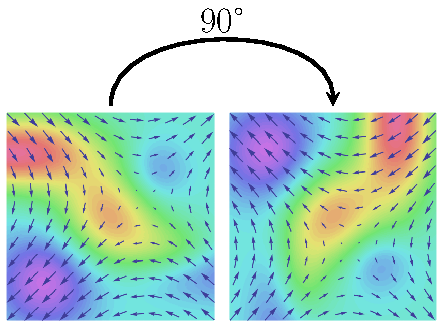
\includegraphics[width=\linewidth]{figures/rotate.pdf}\\ 标量特征（热图）在旋转下不发生变化，而向量特征（箭头）可能改变方向。前述简单的 $\mathrm{E}(3)$ 等变 GNN 没有考虑这一点。}然而，特征 $\vec{f}_u$ 仍按通道处理，并继续假设为在这些变换下不发生变化的\emph{标量}。
%
这限制了该框架能够捕获的空间信息类型。例如，我们可能希望把某些特征编码为\emph{向量}，如点的速度；这些向量在上述变换下\emph{应当}改变方向。
\cite{satorras2021n} 在其架构的一个变体中引入速度概念，部分缓解了这一问题。速度是每个点的一种三维向量属性，会随之正确旋转。然而，这只是 $\mathrm{E}(3)$ 等变网络能够学习的一般表示中的一个很小子空间。一般而言，节点特征可以编码任意维度的\emph{张量}，这些张量仍按照 $\mathrm{E}(3)$ 以明确定义的方式变换。

因此，尽管上述架构已经为许多实际输入表示提供了优雅的等变解决方案，在某些情况下仍有必要探索更广泛的等变函数集合。处理此类设定的现有方法可以分为两类：\emph{不可约表示}（前述层是其简化实例）和\emph{正则表示}。这里仅作简要综述，详细讨论留待未来工作。

\paragraph{不可约表示}
不可约表示建立在如下结论之上：旋转平移群的所有元素都可以化为不可约形式，即由块对角矩阵旋转的向量。关键是，每个块都是一个 \emph{Wigner D-matrix}（即前述球面 CNN 的 Fourier 基）。这类方法使用等变核从一组不可约表示映射到另一组不可约表示。为找出完整的等变映射集合，可以直接求解这些核上的等变约束。所得解是等变基矩阵的线性组合，而这些基矩阵由{\em Clebsch-Gordan 矩阵}和球谐函数导出。

不可约表示方法的早期实例包括 Tensor Field Networks \citep{thomas2018tensor} 和 3D Steerable CNN \citep{weiler20183d}，二者都是在点云上运行的卷积模型。\citet{fuchs2020se} 的 $\mathrm{SE}(3)$-Transformer 使用注意力层而非卷积层，将这一框架扩展到图域。此外，尽管我们的讨论集中于 \citet{satorras2021n} 的特例解，但需要指出，在图上进行旋转或平移等变预测的动机在历史上也曾由其他领域探索，包括用于点云的 Dynamic Graph CNN \citep{wang2019dynamic}，以及用于量子化学的高效消息传递模型，如 SchNet \citep{schutt2018schnet} 和 DimeNet \citep{klicpera2020directional}。

\paragraph{正则表示}
不可约表示方法虽然很有吸引力，却要求直接对底层群表示进行推理，这可能十分繁琐，而且只适用于紧群。正则表示方法更加一般，但会带来额外计算负担——为实现精确等变性，它们需要为\emph{所有}群元素存储潜在特征嵌入的副本\marginnote{事实上，前面各节介绍的群卷积神经网络开创了这一方法。}。

这一领域有一种很有前景的方法，旨在通过指数映射和对数映射的定义考察对 \emph{Lie 群}的等变性，并有望在各种对称群上实现快速原型设计。Lie 群超出了本节范围，读者可参阅这一方向近期两个成功实例：\citet{finzi2020generalizing} 的 LieConv 和 \citet{hutchinson2020lietransformer} 的 LieTransformer。

本节介绍的方法代表了处理几何图上数据的流行方式，并对底层几何具有显式等变性。正如第~\ref{sec:meshes} 节所讨论的，\emph{网格}是几何图的一种特殊实例%， in a way that gives explicit semantics to the \emph{surface} spanned between the nodes.
，可以理解为连续曲面的离散化。
下面将研究网格专用的等变神经网络。


\subsection{内蕴网格 CNN}
网格，尤其是三角网格，是计算机图形学的基本工具，或许也是建模三维对象最常见的方式。深度学习总体上的显著成功，特别是 CNN 在计算机视觉中的成功，使图形学和几何处理社群在 2010 年代中期前后产生了浓厚兴趣\marginnote{
%If $v$ is local, such a description is unique. 
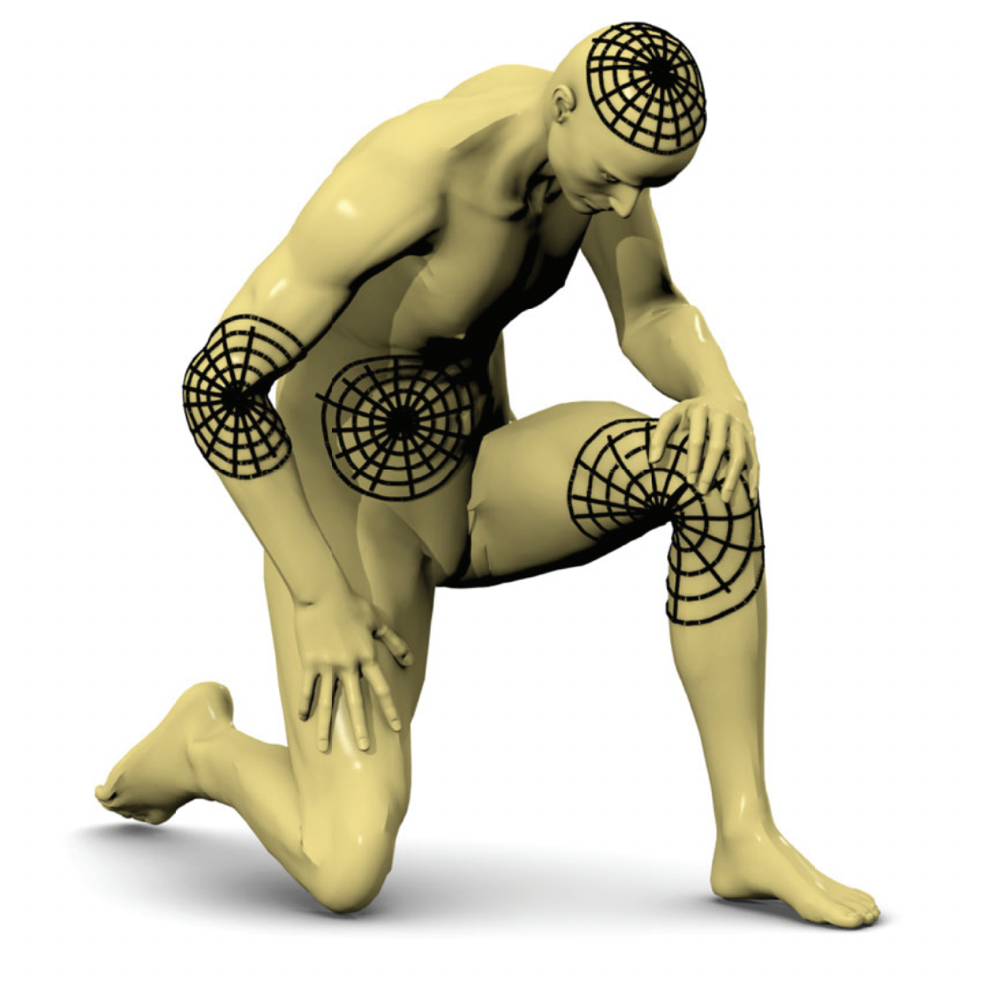
\includegraphics[width=0.9\linewidth]{figures/geo_patch.png}
测地斑块的例子。为使所得斑块成为拓扑圆盘，其半径 $R$ 必须小于单射半径。}，希望为网格数据构建类似架构。


\paragraph{测地斑块}
大多数网格深度学习架构通过
离散化或近似指数映射，并在切平面的坐标系中表示滤波器，来实现形式为~(\ref{eqn:conv_exp}) 的卷积滤波器。
%
发射一条测地线 $\gamma:[0,T]\rightarrow \Omega$，使其从一点 $u=\gamma(0)$ 到达邻近点 $v=\gamma(T)$，可定义一个局部{\em 测地极坐标}系 $(r(u,v),\vartheta(u,v))$，其中 $r$ 是 $u$ 与 $v$ 之间的测地距离（测地线 $\gamma$ 的长度），而 $\vartheta$ 是 $\gamma'(0)$ 与某一局部参考方向之间的夹角。% $X_0(u)$.
%(both tangent vectors in $T_u\Omega$). 
%
由此可以定义{\em 测地斑块} $x(u,r,\vartheta) = x(\exp_u \tilde{\omega}(r,\vartheta))$，其中 $\tilde{\omega}_u: [0,R]\times [0,2\pi) \rightarrow T_u\Omega$ 是局部极坐标标架。




在\marginnote{
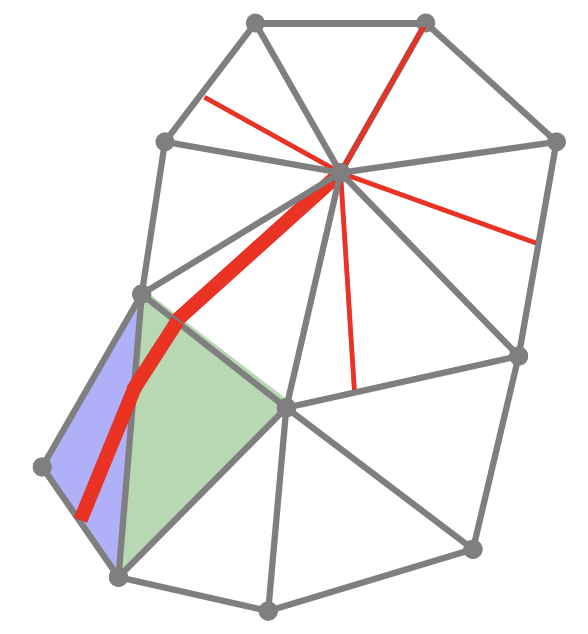
\includegraphics[width=0.9\linewidth]{figures/fmm.png}
网格上离散测地线的构造。}离散化为网格的曲面上，测地线是穿过三角形面的折线。传统上使用 Fast Marching 算法 \cite{kimmel1998computing} 计算测地线；该算法对介质中波传播物理模型里出现的一类非线性 PDE——{\em 程函方程}——进行高效数值近似。\cite{kokkinos2012intrinsic} 调整了这一方案以计算局部测地斑块，随后 \cite{masci2015geodesic} 再次使用它构建{\em Geodesic CNN}，这是首个网格上的内蕴类 CNN 架构。


\paragraph{各向同性滤波器}
重要的是，在测地斑块的定义中，参考方向和斑块定向的选择存在歧义。这恰好就是规范选择的歧义；我们的局部坐标系在相差任意旋转（或角坐标的平移 $x(u,r,\vartheta+\vartheta_0)$）的意义下定义，而该旋转在每个节点处都可能不同。
%
或许最直接的解决方案是使用形式为 $\theta(r)$ 的各向同性滤波器，它以方向无关的方式聚合邻居特征：
$$
(x\star \theta)(u) = \int_0^R \int_0^{2\pi} x(u,r,\vartheta) \theta(r) \mathrm{d}r \mathrm{d}\vartheta.
$$
第~\ref{sec:manifolds}--\ref{sec:meshes} 节讨论的谱滤波器属于这一类别：它们基于各向同性的 Laplacian 算子。
%
然而，这种方法会丢弃重要的方向信息，并且可能无法提取类边缘特征。


\paragraph{固定规范}
另一种方法是{\em 固定某个规范}，第~\ref{sec:manifolds} 节已经提到这一点。\cite{monti2017geometric} 使用主曲率方向：虽然这一选择不是内蕴的，并且在平坦点（曲率为零处）或曲率均匀处（如完美球面上）可能存在歧义，但作者
证明它适合处理近似分片刚性的可变形人体形状。
%
后续工作（例如 \cite{melzi2019gframes}）给出了网格上规范的可靠内蕴构造，即计算内蕴函数的（内蕴）梯度。虽然这类切向量场可能存在奇点（即在某些点处为零），但整个过程对噪声和重新网格化都非常稳健。


\paragraph{角向池化}
\cite{masci2015geodesic} 使用了另一种称为{\em 角向最大池化}的方法。在这种情况下，滤波器 $\theta(r,\vartheta)$ 是各向异性的，但它会在{\em 所有可能的旋转}上与函数进行匹配，随后聚合匹配结果：
$$
(x\star \theta)(u) = \max_{\vartheta_0 \in [0,2\pi) } \,\, \int_0^R \int_0^{2\pi} x(u,r,\vartheta) \theta(r,\vartheta+\vartheta_0) \mathrm{d}r \mathrm{d}\vartheta.
$$
从概念上看，可以将其可视化为用旋转滤波器与测地斑块进行相关运算，并收集最强响应。



%\michael{TBD: discrete}


在网格上，连续积分可以利用一种称为
{\em 斑块算子} \citep{masci2015geodesic} 的构造进行离散化。在节点 $u$ 周围的测地斑块中，邻居节点 $\mathcal{N}_u$\marginnote{通常使用多跳邻居。}在局部极坐标中表示为 $(r_{uv}, \vartheta_{uv})$，并由一组权重函数 $w_1(r,\vartheta), \hdots, w_K(r,\vartheta)$ 加权和聚合（如图~\ref{fig:patches} 所示，它们充当“软像素”）：
%locally aggregating the neighbout node features, 
$$
(x\star \theta)_u = \frac{
\sum_{k=1}^K w_{k} \sum_{v\in \mathcal{N}_u} (r_{uv},\vartheta_{uv}) x_v \, \theta_k
}
{
\sum_{k=1}^K w_{k} \sum_{v\in \mathcal{N}_u} (r_{uv},\vartheta_{uv}) \theta_k
}
$$
  %
  （这里%$x_j$ is the feature at node $j$ and
  $\theta_1,\hdots, \theta_K$ 是滤波器的可学习系数）。多通道特征按通道处理，并配备一族适当的滤波器。
  \cite{masci2015geodesic,boscaini2016learning} 使用预定义权重函数 $w$，而 \cite{monti2017geometric} 进一步允许这些函数可学习。
%




\begin{figure}[h!]
    \centering
    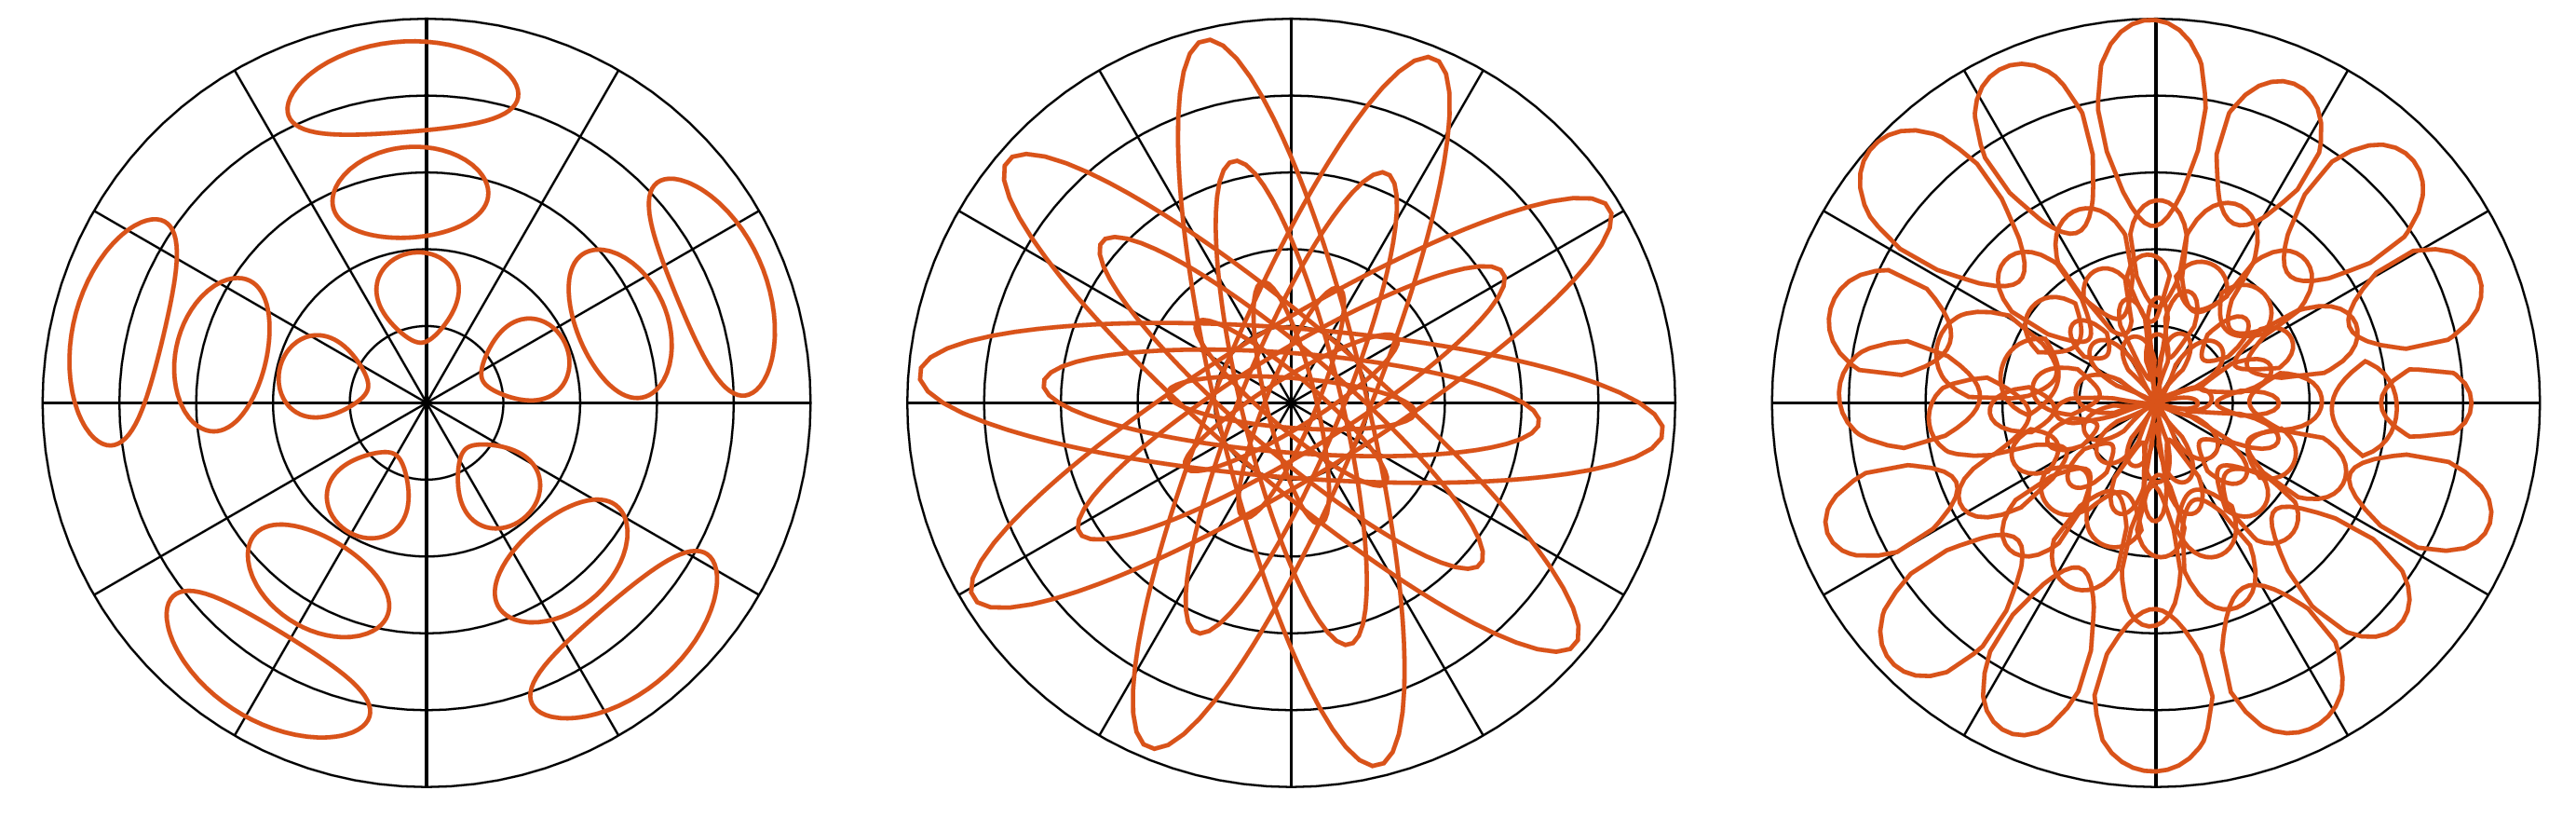
\includegraphics[width=\linewidth]{figures/patch.png}
    \caption{从左到右：Geodesic CNN \citep{masci2015geodesic}、Anisotropic CNN \citep{boscaini2016anisotropic} 和 MoNet \citep{monti2017geometric} 中使用的斑块算子示例，其中权重函数 $w_k(r,\vartheta)$ 的水平集以红色表示。
    }
    \label{fig:patches}
\end{figure}%


%\taco{Since this part of the paper is more focussed on implementation aspects, should we explain how the integrals above are actually evaluated? i.e. how to approximate this one a mesh.}



\paragraph{规范等变滤波器}
各向同性滤波器和角向最大池化都会产生对规范变换{\em 不变}的特征；它们按照平凡表示 $\rho(\fg) = 1$ 进行变换（其中 $\fg \in \mathrm{SO}(2)$ 是局部坐标标架的旋转）。
这一观点启发了 \cite{cohen2019gauge, deHaan2020gauge} 提出的另一种方法，第~\ref{sec:gauges} 节对此进行了讨论。在该方法中，网络计算的特征与任意表示 $\rho$ 相关联，而该表示属于结构群 $\fG$（例如，$\mathrm{SO(2)}$ 或 $\mathrm{O(2)}$ 分别表示坐标标架的旋转群或旋转+反射群）。
%
%For instance, as discussed in Section~\ref{sec:gauges}, a 
切向量按照标准表示 $\rho(\fg) = \fg$ 进行变换。
%(where $\fg$ is viewed as a $2 \times 2$ matrix for a 2D mesh).
再举一例，通过匹配同一滤波器的 $n$ 个旋转副本得到的特征向量，会在规范旋转下通过循环移位进行变换；这称为循环群 $C_n$ 的正则表示。

正如第 \ref{sec:gauges} 节所讨论的，处理这类几何特征（与非平凡表示相关联）时，必须先将它们平行输运到同一向量空间，然后才能应用滤波器。%matching them with a filter.
%
在网格上，可以通过 \cite{deHaan2020gauge} 描述的下列消息传递机制实现这一点。
Let %$u$ denote a mesh node, and 
令 $\mathbf{x}_u \in \R^d$ 为 $d$ 维输入特征，它位于网格节点 $u$ 处。
该特征相对于 $u$ 处（任意）选择的规范表示，并且假设在规范旋转下按照表示 $\rho_{\textup{in}}$ 进行变换，该表示属于 $\fG = \SO{2}$。
类似地，网格卷积的输出特征 $\mathbf{h}_u$
为 $d'$ 维，并且应按照 $\rho_{\textup{out}}$ 进行变换（网络设计者可以任意选择该表示）。


%\michael{Do we use $u$ or $i$ as nodes for meshes? I think $i$ is better to make it compatible with graphs}

与图神经网络类似，我们可以%approximate
通过把消息从邻居 $\mathcal{N}_u$（即 $u$ 的邻居，以及 $u$ 自身）发送给 $u$，在网格上实现规范等变卷积~(\ref{eqn:gauge_eq_conv})：
\begin{equation}
    \mathbf{h}_u = \boldsymbol{\Theta}_{\textup{self}} \; \mathbf{x}_u + \sum_{v \in \mathcal{N}_u} \boldsymbol{\Theta}_{\textup{neigh}}(\vartheta_{uv}) \rho(\fg_{v \rightarrow u}) \mathbf{x}_v,
\end{equation}
其中 $\boldsymbol{\Theta}_{\textup{self}}, \boldsymbol{\Theta}_{\textup{neigh}}(\vartheta_{uv}) \in \R^{d' \times d}$ 是学习得到的滤波器矩阵。%\michael{Not clear: what is the structure of $\rho(\fg_{v \rightarrow u})$, is it a $C\times C$ matrix here? }
结构群元素 $\fg_{v \rightarrow u} \in \SO{2}$ 表示从 $v$ 到 $u$ 的平行输运相对于 $u$ 和 $v$ 处规范所产生的效果，并且可对每个网格预先计算。其作用由\emph{输运矩阵} $\rho(\fg_{v\rightarrow u})\in\mathbb{R}^{d\times d}$ 编码。\marginnote{注意，$d$ 是特征维数，不一定等于网格的维数 2。}
矩阵 $\boldsymbol{\Theta}_{\textup{neigh}}(\vartheta_{uv})$ 依赖于夹角 $\vartheta_{uv}$，即邻居 $v$ 相对于 $u$ 处参考方向（例如标架的第一轴）的角度，因此该核是各向异性的：不同邻居受到不同处理。

正如第 \ref{sec:gauges} 节所解释的，
为使 $\mathbf{h}(u)$ 成为明确定义的几何量，它在规范变换下应变换为 $\mathbf{h}(u) \mapsto \rho_{\textup{out}}(\fg^{-1}(u)) \mathbf{h}(u)$。
当 $\boldsymbol{\Theta}_{\textup{self}} \rho_{\textup{in}}(\vartheta) = \rho_{\textup{out}}(\vartheta) \boldsymbol{\Theta}_{\textup{self}}$ 对所有 $\vartheta \in \SO{2}$ 都成立时，这一条件满足\marginnote{这里略微滥用记号，把二维旋转与角度 $\vartheta$ 等同起来。}；此外还需满足 $\boldsymbol{\Theta}_{\textup{neigh}}(\vartheta_{uv} - \vartheta) \rho_{\textup{in}}(\vartheta) = \rho_{\textup{out}}(\vartheta) \boldsymbol{\Theta}_{\textup{neigh}}(\vartheta_{uv})$。
由于这些约束是线性的，满足约束的矩阵 $\boldsymbol{\Theta}_{\textup{self}}$ 与矩阵值函数 $\boldsymbol{\Theta}_{\textup{neigh}}$ 所构成的空间是线性子空间，因此可以把它们参数化为带可学习系数的基核线性组合：$\boldsymbol{\Theta}_{\textup{self}} = \sum_i \alpha_i \boldsymbol{\Theta}_{\textup{self}}^i$ 以及
$\boldsymbol{\Theta}_{\textup{neigh}} = \sum_i \beta_i \boldsymbol{\Theta}_{\textup{neigh}}^i$。
%similarly for $\boldsymbol{\Theta}_{\textup{neigh}}$.



\subsection{循环神经网络}

迄今为止，我们的讨论始终假设输入在给定域上仅具有\emph{空间}性质。然而，在许多常见用例中，也可以把输入视为\emph{序列}（例如视频、文本或语音）。在这种情况下，我们假设输入由任意多个\emph{步骤}组成；在每个步骤 $t$，给定一个输入信号，并将其表示为 $\vec{X}^{(t)} \in \mathcal{X}(\Omega^{(t)})$。\marginnote{将域视为静态还是动态取决于\emph{时间尺度}：例如，道路网络确实会随时间变化（新道路建成、旧道路拆除），但其变化速度远慢于交通流。类似地，在社交网络中，互动变化（例如 Twitter 用户转发推文）的频率远高于关注图的变化频率。}

虽然一般而言域及其上的信号都可以随时间演化，但通常假设域在所有 $t$ 上保持固定，即 $\Omega^{(t)} = \Omega$。这里将只关注这种情形，但也要指出，例外十分常见。社交网络就是一例：新连接经常建立，旧连接也会消失，因此往往必须考虑域随时间变化。在这种设定下，该域常称为\emph{动态图} \citep{xu2020inductive,rossi2020temporal}。

各个输入 $\vec{X}^{(t)}$ 往往表现出有用的对称性，因此可以用前文讨论的任一架构进行非平凡处理。常见例子包括：\emph{视频}（$\Omega$ 是固定网格，信号是一系列\emph{帧}）；\emph{fMRI 扫描}（$\Omega$ 是表示大脑皮层几何形状的固定\emph{网格}，在所呈现刺激的作用下，不同区域会在不同时间激活）；以及\emph{交通流网络}（$\Omega$ 是表示道路网络的固定\emph{图}，例如在各个节点上记录平均车速）。



假设有一个\emph{编码器}函数 $f(\vec{X}^{(t)})$，它在适合问题的粒度上提供潜在表示，并遵循输入域的对称性。
%
例如\marginnote{该例不失一般性；例如，也可以对时空图上的节点级输出进行等价分析，唯一区别在于编码器 $f$ 的选择（此时它将是置换等变 GNN）。}，考虑处理视频帧：在每个时间步，给定一个以 $n\times d$ 矩阵 $\mathbf{X}^{(t)}$ 表示的\emph{网格结构输入}，其中 $n$ 是像素数（随时间固定），$d$ 是输入通道数（例如 RGB 帧的 $d=3$）。% with a fixed grid.
此外，我们关注整帧层面的分析；此时适合把 $f$ 实现为平移不变 CNN，输出一个 $k$ 维表示 $\vec{z}^{(t)} = f(\vec{X}^{(t)})$，它对应时间步 $t$ 的帧。% $t$ ($\vec{z}\in\mathbb{}^k$).

剩下的任务是\emph{跨所有步骤}恰当地\emph{概括}向量序列 $\vec{z}^{(t)}$。使用\emph{循环神经网络}（RNN）是一种典型方法，它可以在遵循输入时间进程的同时\emph{动态}聚合这些信息，并且容易允许新数据点\emph{在线}到达。\marginnote{注意，向量 $\vec{z}^{(t)}$ 可以视为{\em 时间网格}上的点；因此在某些情况下，也可以用 CNN 处理它们。Transformer 在处理一般序列输入时也日益流行。}
%
%
下面将说明，RNN 本身就是一种值得研究的有趣几何架构，因为它们在输入 $\vec{z}^{(t)}$ 上实现了一种相当不同寻常的对称性。
%RNNs implement, making them an . %Accordingly, we provide an overview of their development here.

\paragraph{SimpleRNN}
\begin{figure}
    \centering
    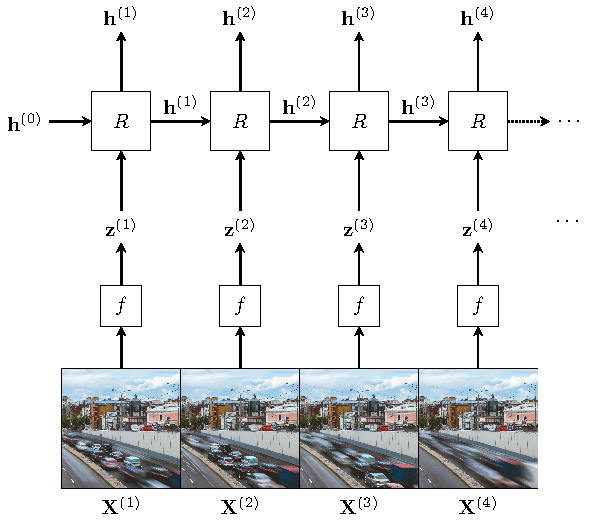
\includegraphics[width=\linewidth]{figures/normal_rnn.pdf}
    \caption{用 RNN 处理视频输入的示意图。每个输入视频帧 $\vec{X}^{(t)}$ 都由共享函数 $f$（例如平移不变 CNN）处理为扁平表示 $\vec{z}^{(t)}$。随后，RNN 更新函数 $R$ 在这些向量上迭代，不断更新概括向量 $\vec{h}^{(t)}$；该向量概括截至且包括 $\vec{z}^{(t)}$ 在内的所有输入。计算以初始概括向量 $\vec{h}^{(0)}$ 为起点，该向量可以预先确定，也可以学习。}
    \label{fig:normal_rnn}
\end{figure}
在每一步，循环神经网络都会计算一个 $m$ 维\emph{概括}向量 $\vec{h}^{(t)}$，用于概括截至且
包括 $t$ 在内的所有输入步骤。这一（部分）概括以当前步骤的
特征和前一步概括为条件，通过共享的\emph{更新}函数 $R : \mathbb{R}^k \times \mathbb{R}^m \rightarrow \mathbb{R}^m$ 按如下方式计算（概览见图 \ref{fig:normal_rnn}）：
\begin{equation}\label{eqn:rnn_upd}
    \vec{h}^{(t)} = R(\vec{z}^{(t)}, \vec{h}^{(t-1)})
\end{equation}
由于 $\vec{z}^{(t)}$ 和 $\vec{h}^{(t-1)}$ 都是\emph{扁平}向量表示，$R$ 最容易表示为单个全连接神经网络层（常称为 \emph{SimpleRNN}\marginnote{尽管名称如此，SimpleRNN 的表示能力非常强。例如，\citet{siegelmann1995computational} 证明这类模型是\emph{图灵完备的}，这意味着它们很可能可以表示我们能够在计算机上执行的\emph{任何}计算。}；见 \citet{elman1990finding,jordan1997serial}）：
\begin{equation}\label{eqn:SimpleRNN}
     \vec{h}^{(t)} = \sigma(\vec{W}\vec{z}^{(t)} + \vec{U}\vec{h}^{(t-1)} + \vec{b})
\end{equation}
其中 $\vec{W}\in\mathbb{R}^{k\times m}$、$\vec{U}\in\mathbb{R}^{m\times m}$ 和 $\vec{b}\in\mathbb{R}^m$ 是可学习参数，$\sigma$ 是激活函数。虽然这会在网络计算图中引入\emph{环}，但实践中
会把网络展开适当的步数，以便应用\emph{随时间反向传播} \citep{robinson1987utility,werbos1988generalization,mozer1989focused}。

随后可以为下游任务恰当利用这些概括向量：如果
需要在序列的每一步进行预测，可以对每个 $\vec{h}^{(t)}$ 分别应用共享预测器。若要对整个序列分类，通常把最终概括 $\vec{h}^{(T)}$ 传给分类器。这里，$T$ 是序列长度。

特别地，初始概括向量通常设为零向量，即 $\vec{h}^{(0)}=\vec{0}$，或者设为可学习。分析初始概括向量的设定方式，还可以推导出 RNN 所表现的一种有趣\emph{平移等变性}。

\paragraph{RNN 中的平移等变性}由于我们把各个步骤 $t$ 解释为\emph{离散时间步}，输入向量 $\vec{z}^{(t)}$ 可以看作位于一维时间步\marginnote{注意，该构造可以扩展到更高维网格，从而例如以\emph{扫描线}方式处理图像上的信号。该构造支撑了一系列流行模型，如 \citet{van2016pixel} 的 PixelRNN。}\emph{网格}上。虽然尝试把 CNN 的平移等变性分析扩展到这里很有吸引力，但不能直接做到这一点。

为说明原因，假设把序列向左平移一步，得到新序列 $\vec{z}'^{(t)} = \vec{z}^{(t+1)}$。%, recovering a new sequence $\vec{z}'^{(t)} = \vec{z}^{(t+1)}$.
按照平移等变性的预期，我们可能会尝试证明 $\vec{h}'^{(t)} = \vec{h}^{(t+1)}$，但这一般不成立。考虑 $t = 1$；直接应用并展开更新函数可得：
\begin{align}\label{eqn:shiftrnn}
    \vec{h}'^{(1)} &= R(\vec{z}'^{(1)}, \vec{h}^{(0)}) = R(\vec{z}^{(2)}, \vec{h}^{(0)})\\ 
    \vec{h}^{(2)} &= R(\vec{z}^{(2)}, \vec{h}^{(1)}) = R(\vec{z}^{(2)}, R(\vec{z}^{(1)}, \vec{h}^{(0)}))\label{eqn:shiftrnn2} 
\end{align}
因此，除非能保证 $\vec{h}^{(0)} = R(\vec{z}^{(1)}, \vec{h}^{(0)})$，否则无法得到平移等变性。随后可以对步骤 $t > 1$ 进行类似分析。

所幸，只需稍微调整 $\vec{z}$ 的表示方式并适当选择 $R$，就可以满足上述等式，从而给出 RNN 对平移等变的一种设定。
%
问题主要出在\emph{边界条件}：上述等式包含 $\vec{z}^{(1)}$，而左移操作破坏了它。为抽象掉这一问题，我们考察 RNN 如何处理经过适当\emph{左填充}的序列 $\bar{\vec{z}}^{(t)}$，其定义如下：
$$
    \bar{\vec{z}}^{(t)} = \begin{cases}
        \vec{0} & t \leq t'\\
        \vec{z}^{(t - t')} & t > t' 
    \end{cases}
$$
现在，这种序列允许最多左移\marginnote{注意，如果使用不同于 $\vec{0}$ 的填充向量，也会得到等价分析。}$t'$ 步，而不破坏任何原始输入元素。此外，无需单独处理右移；事实上，对右移的等变性自然可以从 RNN 方程推出。

现在可以再次分析 RNN 在 $\bar{\vec{z}}^{(t)}$ 左移版本上的运算，将其记为 $\bar{\vec{z}}'^{(t)} = \bar{\vec{z}}^{(t+1)}$，正如式 \ref{eqn:shiftrnn}--\ref{eqn:shiftrnn2} 中所做的那样：
\begin{align*}
    \vec{h}'^{(1)} &= R(\bar{\vec{z}}'^{(1)}, \vec{h}^{(0)}) = R(\bar{\vec{z}}^{(2)}, \vec{h}^{(0)})\\ \vec{h}^{(2)} &= R(\bar{\vec{z}}^{(2)}, \vec{h}^{(1)}) = R(\bar{\vec{z}}^{(2)}, R(\bar{\vec{z}}^{(1)}, \vec{h}^{(0)})) = R(\bar{\vec{z}}^{(2)}, R(\vec{0}, \vec{h}^{(0)}))
\end{align*}
替换 $\bar{\vec{z}}^{(1)} = \vec{0}$ 在 $t' \geq 1$ 时成立，即只要应用了任何填充便成立\marginnote{与此非常类似，可以推导出对左移 $s$ 步的等变性，只要 $t' \geq s$。}。现在，可以保证对左移一步的等变性（$\vec{h}'^{(t)} = \vec{h}^{(t+1)}$），只要 $\vec{h}^{(0)} = R(\vec{0}, \vec{h}^{(0)})$。


换言之，必须把 $\vec{h}^{(0)}$ 选为函数 $\gamma(\vec{h}) = R(\vec{0}, \vec{h})$ 的\emph{不动点}。如果恰当地选择更新函数 $R$，不仅可以保证这类不动点存在，甚至可以反复应用 $R$ 直至收敛，直接获得它们；例如：
\begin{equation}\label{eqn:iterated}
    \vec{h}_0 = \vec{0} \qquad \vec{h}_{k+1} = \gamma(\vec{h}_{k}),
\end{equation}
%
其中，索引 $k$ 表示计算中 $R$ 的迭代次数，与表示 RNN 时间步的索引 $(t)$ 相区别。
%
若选择 $R$ 使 $\gamma$ 成为\emph{压缩映射}\marginnote{压缩映射是如下函数 $\gamma: \mathcal{X}\rightarrow \mathcal{X}$：在某个范数 $\|\cdot\|$（定义于 $\mathcal{X}$ 上）下，应用 $\gamma$ 会\emph{压缩}点之间的距离；即对于所有 $\vec{x},\vec{y}\in\mathcal{X}$ 以及某个 $q\in [0,1)$，均有 $\|\gamma(\vec{x}) - \gamma(\vec{y})\| \leq q\|\vec{x} - \vec{y}\|$。反复迭代这类函数必然收敛到唯一不动点，这是 \emph{Banach 不动点定理} \citep{banach1922operations} 的直接推论。}，那么这种迭代确实会收敛到\emph{唯一}不动点。因此，可以迭代式~(\ref{eqn:iterated}) 直至 $\vec{h}_{k+1} = \vec{h}_k$，并令 $\vec{h}^{(0)} = \vec{h}_k$。注意，这一计算等价于用“足够多”的零向量对序列进行\emph{左填充}。

\paragraph{RNN 的深度}
堆叠多个 RNN 也很容易：只需把向量 $\vec{h}^{(t)}$ 作为第二个 RNN 的输入序列。这种构造有时称为“深层 RNN”，但这一名称可能产生误导。实际上，由于循环运算被反复应用，即便单个 RNN“层”的深度也\emph{等于输入步骤数}。

这通常会在优化 RNN 时引入格外棘手的学习动力学，因为每个训练样本都会对更新网络的\emph{共享}参数产生多次梯度更新。这里将关注其中或许最突出的问题——\emph{梯度消失}与\emph{梯度爆炸} \citep{bengio1994learning}。鉴于 RNN 的深度和参数共享，这一问题在 RNN 中尤其严重，并且单独推动了若干最有影响力的 RNN 研究。更详细的概述见 \citet{pascanu2013difficulty}；该工作深入研究了 RNN 的训练动力学，并从分析、几何和动力系统等多种视角揭示了这些挑战。

为说明梯度消失，考虑采用 S 形激活函数 $\sigma$ 的 SimpleRNN\marginnote{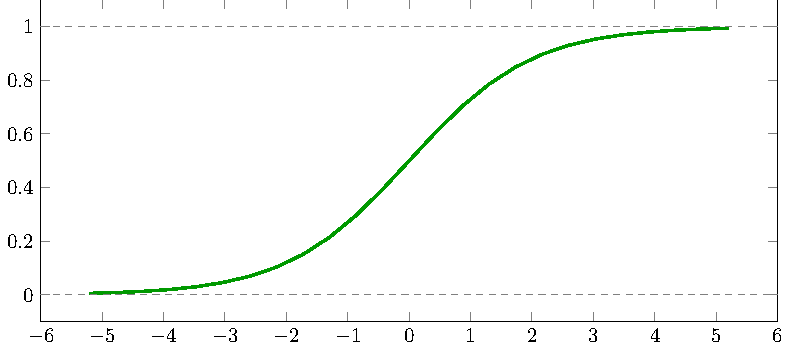
\includegraphics[width=\linewidth]{figures/sigmoid.pdf}\\ 这类激活函数包括\emph{logistic 函数} $\sigma(x) = \frac{1}{1+\exp(-x)}$ 和\emph{双曲正切} $\sigma(x)=\tanh x$。它们的图像具有鲜明的 S 形，因而称为 S 形函数。}，其导数绝对值 $|\sigma'|$ 始终介于 $0$ 与 $1$ 之间。许多个这样的值相乘，会使梯度迅速趋于零，这意味着输入序列中的早期步骤可能完全无法影响网络参数的更新。

例如，考虑下一词预测任务（常见于预测键盘等场景）和输入文本\emph{“Petar 是塞尔维亚人。他出生于 \dots [长段落] \dots Petar 目前居住在 \rule{1.3cm}{0.15mm}”}。这里，只有考虑段落最开头，才能合理推断下一个词是“塞尔维亚”；但梯度传播到这一输入步骤时很可能已经消失，使得从这类样本中学习非常困难。

深度前馈神经网络也曾受到梯度消失问题困扰，直到 ReLU 激活函数出现（其梯度\emph{恰好}等于零或一，因而解决了梯度消失问题）。然而，在 RNN 中使用 ReLU 很容易导致\emph{梯度爆炸}，因为更新函数的输出空间此时\emph{无界}，而梯度下降会为每个输入步骤更新一次单元，使更新量级迅速累积。
%
从历史上看，梯度消失现象很早就被视为使用循环网络的一项重大障碍。应对这一问题推动了更复杂 RNN 层的发展，下面将对其进行介绍。


\subsection{长短期记忆网络}
\label{sec:lstm}

\begin{figure}
    \centering
    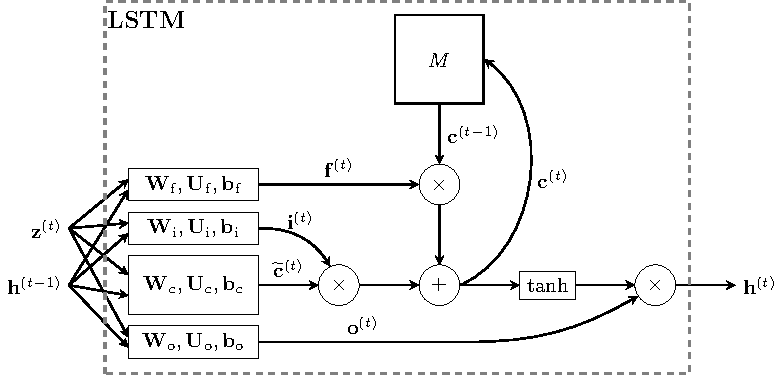
\includegraphics[width=\linewidth]{figures/lstm.pdf}
    \caption{长短期记忆（LSTM）的数据流，其中各组成部分和记忆单元（$M$）均清晰标出。根据当前输入 $\vec{z}^{(t)}$、前一概括 $\vec{h}^{(t-1)}$ 和前一单元状态 $\vec{c}^{(t-1)}$，LSTM 预测更新后的单元状态 $\vec{c}^{(t)}$ 和概括 $\vec{h}^{(t)}$。}
    \label{fig:lstm}
\end{figure}
显著减轻 RNN 中梯度消失影响的一项关键发明是\emph{门控机制}，它允许网络以数据驱动方式选择性地\emph{覆写}信息。这类\emph{门控 RNN} 的著名实例包括{\em 长短期记忆}（LSTM；\citet{hochreiter1997long}）和{\em 门控循环单元}（GRU；\citet{cho2014learning}）。为说明此类模型的运算，这里主要讨论 LSTM，具体采用 \citet{graves2013generating} 提出的变体。LSTM 中的概念很容易推广到其他门控 RNN。

阅读本节时，参照图 \ref{fig:lstm} 可能会有所帮助；该图展示了正文将讨论的全部 LSTM 运算。

LSTM 通过引入\emph{记忆单元}来扩展循环计算；该单元存储在计算步骤之间得到\emph{保留}的\emph{单元状态}向量 $\vec{c}^{(t)}\in\mathbb{R}^m$。LSTM 计算概括向量 $\vec{h}^{(t)}$，直接以 $\vec{c}^{(t)}$ 为依据，而 $\vec{c}^{(t)}$ 又使用 $\vec{z}^{(t)}$、$\vec{h}^{(t-1)}$ 和 $\vec{c}^{(t-1)}$ 计算。
关键在于，单元\textbf{不会}根据 $\vec{z}^{(t)}$ 和 $\vec{h}^{(t-1)}$ 被完全覆写，否则网络将面临与 SimpleRNN 相同的问题。相反，可以\emph{保留}一定比例的前一单元状态，而这一比例由数据显式\emph{学习}得到。

与 SimpleRNN 一样，我们在当前输入步骤和前一概括上使用单个全连接神经网络层计算特征：\marginnote{注意，这里把激活函数设为 $\tanh$；由于 LSTM 旨在缓解梯度消失问题，此时使用 S 形激活函数是合适的。}
\begin{equation}\label{eqn:lstmstart}
     \widetilde{\vec{c}}^{(t)} = \tanh(\vec{W}_c\vec{z}^{(t)} + \vec{U}_c\vec{h}^{(t-1)} + \vec{b}_c)
\end{equation}
但是，如前所述，我们不允许该向量的\emph{全部}分量进入单元，因此称它为\emph{候选}特征向量，并记为 $\widetilde{\vec{c}}^{(t)}$。LSTM 转而直接学习\emph{门控向量}；它们是范围 $[0, 1]$ 内的实值向量，用于决定允许多少信号进入、离开和覆写记忆单元。

一共计算三个这样的门，它们都基于 $\vec{z}^{(t)}$ 和 $\vec{h}^{(t-1)}$：\emph{输入门} $\vec{i}^{(t)}$ 计算允许进入单元的候选向量比例；\emph{遗忘门} $\vec{f}^{(t)}$ 计算要保留的前一单元状态比例；\emph{输出门} $\vec{o}^{(t)}$ 计算用于最终概括向量的新单元状态比例。通常，所有这些门也通过单个全连接层得到，但使用\emph{logistic sigmoid} 激活 $\mathrm{logistic}(x) = \frac{1}{1+\exp(-x)}$，以保证输出位于 $[0, 1]$ 范围内\marginnote{注意，这三个门本身是\emph{向量}，即 $\vec{i}^{(t)}, \vec{f}^{(t)}, \vec{o}^{(t)}\in [0,1]^m$。这使它们能够控制 $m$ 个维度中的\emph{每一个}有多少分量可通过门。}：
\begin{align}\label{eqn:lstm_gate}
     \vec{i}^{(t)} &= \mathrm{logistic}(\vec{W}_\mathrm{i}\vec{z}^{(t)} + \vec{U}_\mathrm{i}\vec{h}^{(t-1)} + \vec{b}_\mathrm{i})\\
     \vec{f}^{(t)} &= \mathrm{logistic}(\vec{W}_\mathrm{f}\vec{z}^{(t)} + \vec{U}_\mathrm{f}\vec{h}^{(t-1)} + \vec{b}_\mathrm{f})\\
     \vec{o}^{(t)} &= \mathrm{logistic}(\vec{W}_\mathrm{o}\vec{z}^{(t)} + \vec{U}_\mathrm{o}\vec{h}^{(t-1)} + \vec{b}_\mathrm{o})
\end{align}

最后，恰当地应用这些门以解码\emph{新的}单元状态 $\vec{c}^{(t)}$，再由输出门对其调制以产生概括向量 $\vec{h}^{(t)}$，如下所示：
\begin{align}
    \vec{c}^{(t)} &= \vec{i}^{(t)}\odot\widetilde{\vec{c}}^{(t)} + \vec{f}^{(t)}\odot\vec{c}^{(t-1)}\\
    \vec{h}^{(t)} &= \vec{o}^{(t)}\odot\tanh(\vec{c}^{(t)})\label{eqn:lstm_end}
\end{align}
其中 $\odot$ 表示向量逐元素乘法。式 (\ref{eqn:lstmstart})--(\ref{eqn:lstm_end}) 共同完整指定了 LSTM 的\emph{更新规则}，该规则现在还考虑单元向量 $\vec{c}^{(t)}$\marginnote{这仍与式 (\ref{eqn:rnn_upd}) 的 RNN 更新蓝图兼容；只需把概括向量视为 $\vec{h}^{(t)}$ 和 $\vec{c}^{(t)}$ 的\emph{拼接}，有时记为 $\vec{h}^{(t)}\|\vec{c}^{(t)}$。}：
$$
    (\vec{h}^{(t)}, \vec{c}^{(t)}) = R(\vec{z}^{(t)}, (\vec{h}^{(t-1)}, \vec{c}^{(t-1)}))
$$
注意，由于 $\vec{f}^{(t)}$ 的值由 $\vec{z}^{(t)}$ 和 $\vec{h}^{(t-1)}$ 得到，因而可直接从数据中\emph{学习}，LSTM 实际上学会了如何恰当地遗忘过去的经验。事实上，$\vec{f}^{(t)}$ 的值直接出现在所有 LSTM 参数（$\vec{W}_*, \vec{U}_*, \vec{b}_*$）的反向传播更新中，使网络能够以数据驱动方式显式\emph{控制}梯度跨时间步消失的程度。

除了直接应对梯度消失问题外，门控 RNN 还带来一种非常有用的对\emph{时间扭曲}变换的不变性，而 SimpleRNN 无法获得这种性质。

\paragraph{门控 RNN 的时间扭曲不变性}我们首先在\emph{连续时间}设定下说明\marginnote{之所以关注连续设定，是因为在其中更容易对时间操作进行推理。}\emph{扭曲时间}意味着什么，以及循环模型要对这类变换实现不变性需要满足哪些条件。我们的论述主要遵循 \citet{tallec2018can} 的工作；该工作最初描述了这一现象，而且确实是最早从不变性视角研究 RNN 的工作之一。

假设有一个连续时域信号 $z(t)$，我们希望在其上应用 RNN。为使 RNN 对概括向量 $\vec{h}^{(t)}$ 的离散时间计算\marginnote{我们用 $h(t)$ 表示时间 $t$ 的连续信号，用 $\vec{h}^{(t)}$ 表示时间步 $t$ 的离散信号。}与连续域中的对应量 $h(t)$ 对齐，考察其线性 Taylor 展开：
\begin{equation}
    h(t + \delta) \approx h(t) + \delta\frac{\mathrm{d}h(t)}{\mathrm{d}t}
\end{equation}
令 $\delta = 1$，便可恢复 $h(t)$ 与 $h(t+1)$ 之间的关系，这正是 RNN 更新函数 $R$（式 \ref{eqn:rnn_upd}）所计算的内容。具体而言，RNN 更新函数满足下列微分方程：
\begin{equation}\label{eqn:ode_pre_warp}
    \frac{\mathrm{d}h(t)}{\mathrm{d}t} = h(t+1) - h(t) = R(z(t+1), h(t)) - h(t)
\end{equation}

我们希望 RNN 对信号的采样方式（例如改变时间计量单位）具有稳健性，以适应其中的任何缺陷或不规则性。形式上，我们把\emph{时间扭曲}\marginnote{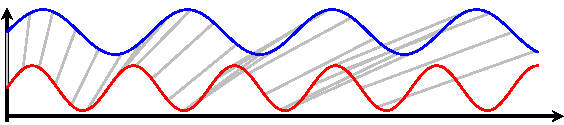
\includegraphics[width=\linewidth]{figures/time_warp.pdf}\\ 这类扭曲运算可以很\emph{简单}，例如时间重缩放；如上图所示的 $\tau(t) = 0.7t$，在离散设定下相当于每隔 $\sim 1.43$ 步接收一个新输入。不过，它也允许各种\emph{可变}采样率，例如采样可以在整个时域中自由加速或减速。}运算 $\tau : \mathbb{R}^+\rightarrow\mathbb{R}^+$ 定义为时间之间任意单调递增的可微映射。之所以选择记号 $\tau$，是因为时间扭曲表示时间的一个\emph{自同构}。

进一步地，如果对于该类中的任意模型和任意这样的 $\tau$，都存在该类中的另一个模型（可能是同一个模型），能够以原模型处理未扭曲数据的相同方式处理扭曲后的数据，我们就称这一模型类对时间扭曲\emph{不变}。

这是一项可能非常有用的性质。如果某个 RNN 类能够很好地建模短期依赖，并且可以证明该类对时间扭曲不变，那么就知道可以通过训练使这类模型也有效捕获长期依赖（因为长期依赖对应于对具有短期依赖的信号进行时间膨胀扭曲）。
%
下文很快会看到，LSTM 等\emph{门控} RNN 模型被提出用于建模长程依赖并非巧合。实现时间扭曲不变性与门控机制的存在紧密相关，例如 LSTM 的输入门、遗忘门和输出门。

当时间由 $\tau$ 扭曲时，RNN 在时间 $t$ 观察到的信号是 $z(\tau(t))$；为了对这类扭曲保持不变，它应预测经过等价扭曲的概括函数 $h(\tau(t))$。再次使用 Taylor 展开，可以推导出式 \ref{eqn:ode_pre_warp} 在扭曲时间下的形式，RNN 更新 $R$ 应满足该形式：
\begin{equation}\label{eqn:ode_post_warp}
    \frac{\mathrm{d}h(\tau(t))}{\mathrm{d}\tau(t)} = R(z(\tau(t+1)), h(\tau(t))) - h(\tau(t))
\end{equation}
然而，上述导数是相对于扭曲时间 $\tau(t)$ 计算的，因此没有考虑原始信号。为使模型显式考虑扭曲变换，需要相对于 $t$ 对扭曲后的概括函数求导。应用链式法则得到下列微分方程：
\begin{equation}\label{eqn:full_ode_warp}
    \frac{\mathrm{d}h(\tau(t))}{\mathrm{d}t} = \frac{\mathrm{d}h(\tau(t))}{\mathrm{d}\tau(t)}\frac{\mathrm{d}\tau(t)}{\mathrm{d}t} = \frac{\mathrm{d}\tau(t)}{\mathrm{d}t}R(z(\tau(t+1)), h(\tau(t))) - \frac{\mathrm{d}\tau(t)}{\mathrm{d}t}h(\tau(t))
\end{equation}
而且，为使（连续时间）RNN 对\emph{任意}时间扭曲 $\tau(t)$ 保持不变，它必须能够显式表示导数 $\frac{\mathrm{d}\tau(t)}{\mathrm{d}t}$，但我们并不假设事先知道该导数！因此需要引入一个近似此导数的\emph{可学习}函数 $\Gamma$。例如，$\Gamma$ 可以是考虑 $z(t+1)$ 和 $h(t)$ 并预测标量输出的神经网络。

现在注意，从时间扭曲下的\emph{离散} RNN 模型视角看，其输入 $\vec{z}^{(t)}$ 对应于 $z(\tau(t))$，其概括 $\vec{h}^{(t)}$ 对应于 $h(\tau(t))$。为获得 $\vec{h}^{(t)}$ 与 $\vec{h}^{(t+1)}$ 之间保持时间扭曲不变性所需的关系，我们对 $h(\tau(t))$ 进行一步 Taylor 展开：
\begin{equation*}
    h(\tau(t + \delta)) \approx h(\tau(t)) + \delta\frac{\mathrm{d}h(\tau(t))}{\mathrm{d}t}
\end{equation*}
再次令 $\delta=1$，代入式 \ref{eqn:full_ode_warp}，然后离散化：
\begin{align*}
    \vec{h}^{(t+1)} &= \vec{h}^{(t)} + \frac{\mathrm{d}\tau(t)}{\mathrm{d}t}R(\vec{z}^{(t+1)}, \vec{h}^{(t)}) - \frac{\mathrm{d}\tau(t)}{\mathrm{d}t}\vec{h}^{(t)}\\
    &= \frac{\mathrm{d}\tau(t)}{\mathrm{d}t}R(\vec{z}^{(t+1)}, \vec{h}^{(t)}) + \left(1 - \frac{\mathrm{d}\tau(t)}{\mathrm{d}t}\right)\vec{h}^{(t)}
\end{align*}
最后，把 $\frac{\mathrm{d}\tau(t)}{\mathrm{d}t}$ 替换为前述可学习函数 $\Gamma$。由此得到时间扭曲不变 RNN 所需的形式：
\begin{equation}\label{eqn:GaRNN}
    \vec{h}^{(t+1)} = \Gamma(\vec{z}^{(t+1)}, \vec{h}^{(t)})R(\vec{z}^{(t+1)}, \vec{h}^{(t)}) + (1 - \Gamma(\vec{z}^{(t+1)}, \vec{h}^{(t)}))\vec{h}^{(t)}
\end{equation}
可以很快推断，SimpleRNN（式 \ref{eqn:SimpleRNN}）\emph{不}具有时间扭曲不变性，因为它们不包含式 \ref{eqn:GaRNN} 中的第二项。相反，$\vec{h}^{(t)}$ 被 $R(\vec{z}^{(t+1)}, \vec{h}^{(t)})$ 完全覆写，这对应于假设根本没有时间扭曲，即 $\frac{\mathrm{d}\tau(t)}{\mathrm{d}t} = 1$，也就是 $\tau(t) = t$。

此外，连续时间 RNN 与基于 $R$ 的离散 RNN 之间的联系依赖于 Taylor 近似的准确性，而只有时间扭曲导数不太大时该近似才成立，即 $\frac{\mathrm{d}\tau(t)}{\mathrm{d}t}\lesssim 1$。直观解释如下：如果时间扭曲运算以某种方式\emph{压缩时间}，使时间增量（$t \rightarrow t + 1$）大到无法采样中间的数据变化，那么模型永远不可能以处理原始输入的相同方式处理时间扭曲输入，因为它根本无法获得相同信息。相反，我们的框架完全允许任何形式的时间\emph{膨胀}（在离散意义下，这对应于在输入时间序列中插入零）。

结合 $\tau$ 单调递增这一要求（$\frac{\mathrm{d}\tau(t)}{\mathrm{d}t} > 0$），可以把 $\Gamma$ 的输出空间限制为 $0 < \Gamma(\vec{z}^{(t+1)}, \vec{h}^{(t)}) < 1$，这促使我们为 $\Gamma$ 使用 logistic sigmoid 激活，例如：
$$
    \Gamma(\vec{z}^{(t+1)}, \vec{h}^{(t)}) = \mathrm{logistic}({\bf W}_\Gamma\vec{z}^{(t+1)} + {\bf U}_\Gamma\vec{h}^{(t)} + \vec{b}_\Gamma)
$$
这与 LSTM 门控方程\emph{完全}一致（例如式 \ref{eqn:lstm_gate}）。主要区别在于，LSTM 计算门控\emph{向量}，而式 \ref{eqn:GaRNN} 意味着 $\Gamma$ 应输出标量。向量化门 \citep{hochreiter1991untersuchungen} 允许在 $\vec{h}^{(t)}$ 的每个维度拟合\emph{不同的}扭曲导数，从而同时对\emph{多个}时间跨度进行推理。

这里有必要稍作停顿，总结已经完成的工作。通过要求 RNN 类对（非破坏性）时间扭曲不变，我们推导出它必须具有的必要形式（式 \ref{eqn:GaRNN}），并证明该形式恰好对应于\emph{门控} RNN 类。在这一视角下，门的主要作用是准确拟合扭曲变换的\emph{导数} $\frac{\mathrm{d}\tau(t)}{\mathrm{d}t}$。

\emph{类不变性}的概念与此前研究的不变性有所不同。也就是说，一旦在采用 $\tau_1(t)$ 时间扭曲的输入上训练了门控 RNN，通常不能将其零样本迁移\marginnote{可以进行零样本迁移的一种情形是，假设第二次时间扭曲是第一次的\emph{时间重缩放}（$\tau_2(t) = \alpha\tau_1(t)$）。把在 $\tau_1$ 上预训练的门控 RNN 迁移到由 $\tau_2$ 扭曲的信号，只需\emph{重缩放门}：$\Gamma_2(\vec{z}^{(t+1)}, \vec{h}^{(t)}) = \alpha \Gamma_1(\vec{z}^{(t+1)}, \vec{h}^{(t)})$。$R$ 可以保留其参数（$R_1 = R_2$）。}到由不同 $\tau_2(t)$ 扭曲的信号。相反，类不变性只保证门控 RNN 具有足够的表达能力，能以相同方式拟合这两个信号，但其模型参数可能大不相同。尽管如此，有效门控机制与拟合扭曲导数紧密相关这一认识，可以为门控 RNN 优化提供有用准则，下面作简要说明。

例如，通常可以假设，我们希望在信号中跟踪的依赖关系跨度位于 $[T_l, T_h]$ 个时间步的范围内。

通过分析式 \ref{eqn:full_ode_warp} 的解析解，可以证明，门控 RNN 对 $\vec{h}^{(t)}$ 的特征\emph{遗忘时间}与 $\frac{1}{\Gamma(\vec{z}^{(t+1)}, \vec{h}^{(t)})}$ 成正比。因此，为了有效记住假设范围内的信息，我们希望门控值位于 $\left[\frac{1}{T_h}, \frac{1}{T_m}\right]$ 之间。

进一步地，若假设 $\vec{z}^{(t)}$ 和 $\vec{h}^{(t)}$ 大致\emph{以零为中心}——这是应用层归一化 \citep{ba2016layer} 等变换时常见的副产物——则可以假设 $\mathbb{E}[\Gamma(\vec{z}^{(t+1)}, \vec{h}^{(t)})] \approx \mathrm{logistic}(\vec{b}_\Gamma)$。因此，控制门控机制的\emph{偏置}向量是控制有效门值的一种非常有力的方法\marginnote{\citet{gers2000recurrent,jozefowicz2015empirical} 已经发现这一洞见，并根据经验建议把 LSTM 的遗忘门偏置初始化为常数正向量，例如 $\vec{1}$。}。

结合上述两个观察，可以得出结论：通过初始化 $\vec{b}_\Gamma\sim-\log(\mathcal{U}(T_l, T_h) - 1)$ 可以获得合适范围的门控值，其中 $\mathcal{U}$ 是实数均匀分布。\citet{tallec2018can} 将这一建议称为\emph{时间尺度初始化}，经验证明它可以改善门控 RNN 对长程依赖的建模。

\paragraph{使用 RNN 的序列到序列学习}
使用 RNN 支撑计算的一个著名历史实例是\emph{序列到序列}翻译任务，例如自然语言的{\em 机器翻译}。\citet{sutskever2014sequence} 开创性的 \emph{seq2seq} 工作把概括向量 $\vec{h}^{(T)}$ 作为\emph{解码器} RNN 的初始输入，并把 RNN 模块的输出作为下一步输入，从而实现了这一目标。

\begin{figure}
    \centering
    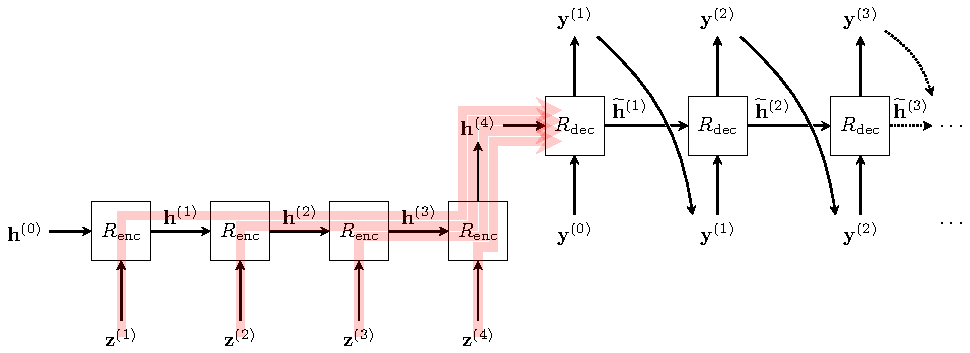
\includegraphics[width=\linewidth]{figures/bottle_rnn.pdf}
    \caption{seq2seq 架构的一个典型实例，包含 RNN 编码器 $R_\mathrm{enc}$ 和 RNN 解码器 $R_\mathrm{dec}$。解码器以编码器输出的最终概括向量 $\vec{h}^{(T)}$ 为初始状态，然后以\emph{自回归}方式运行：在每一步，前一步的预测输出都作为输入反馈给 $R_\mathrm{dec}$。红线还示意了瓶颈问题：概括向量 $\vec{h}^{(T)}$ 被迫存储翻译输入序列所需的\emph{全部}相关信息，随着输入长度增加，这一点会越来越困难。}
    \label{fig:rnn_bottleneck}
\end{figure}

这给概括向量 $\vec{h}^{(T)}$ 带来了巨大的表示压力。在深度学习语境下，$\vec{h}^{(T)}$ 有时称为\emph{瓶颈}\marginnote{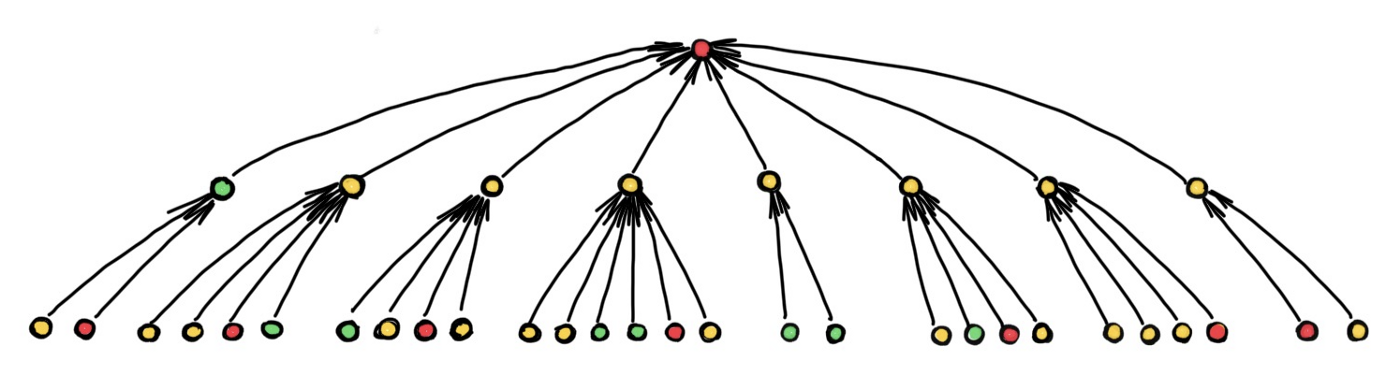
\includegraphics[width=\linewidth]{figures/bottleneck.png}\\
瓶颈效应最近在图表示学习社群 \citep{alon2020bottleneck} 以及神经算法推理领域 \citep{cappart2021combinatorial} 受到广泛关注。}。它的固定容量必须足以表示整个输入序列的内容，其表示方式还要有利于生成相应序列，同时支持长度相差很大的输入序列（图 \ref{fig:rnn_bottleneck}）。

实际上，输出的不同步骤可能希望聚焦（\emph{关注}）输入的不同部分，而所有这些选择都难以通过瓶颈向量表示。基于这一观察，\citet{bahdanau2014neural} 提出了流行的\emph{循环注意力}模型。在处理的每一步，RNN 都会生成一个\emph{查询向量}；该查询向量随后与\emph{每个}时间步的表示 $\vec{h}^{(t)}$ 交互，主要方式是对它们计算加权和。该模型开创了神经内容注意力，并早于 Transformer 模型的成功。

最后，虽然注意力提供了一种动态聚焦输入内容各部分的\emph{软}方式，大量工作也学习了以更\emph{显式}的方式把注意力指向输入。\citet{vinyals2015pointer} 的\emph{指针网络}是一种具有算法依据的有力方法：它对循环注意力作简单修改，从而允许指向\emph{大小可变}输入中的元素。随后，这些结论被推广到 \emph{set2set} 架构 \citep{vinyals2016order}；该架构借助由指针网络支撑的 LSTM，把 seq2seq 模型推广到无序集合。
